\documentclass{beamer}

\usepackage[italian]{babel}
\usepackage{amsmath, amssymb}
\usepackage{amsthm}
\usepackage{amstext}
\usepackage{array}
\usepackage{graphicx,color,psfrag,pgfplots}
\usepackage[bf,footnotesize,center]{caption}
\captionsetup{labelformat=empty,labelsep=none}
\usepackage[tight]{subfigure}
\usepackage{bbm}
\usepackage{tikz}
\usetikzlibrary{patterns,shapes,positioning,arrows,calc,shadows}

\newcommand{\vect}[1]{\mathbf{#1}}
\newcommand{\figref}[1]{( Fig.\ref{#1} )}

\theoremstyle{plain}
\newtheorem{teorema}{Teorema}

\graphicspath{{img/}}

%Comando per togliere le etichette dal subfigure
\renewcommand{\thesubfigure}{}
\makeatletter
\renewcommand{\p@subfigure}{}
\renewcommand{\@thesubfigure}{\thesubfigure\hskip\subfiglabelskip}
\makeatother
%--------------

% Tema
\usetheme{MY-CambridgeUS}

\author[Bortolossi]{Andrea Bortolossi}
\title[WIP]{Work in progress}
\institute[Polimi\&Micron]{Politecnico di Milano - Micron Technology}
\DeclareGraphicsExtensions{.eps}
\titlegraphic{
\begin{center}
\begin{columns}
\begin{column}{0.5 \paperwidth}
\begin{center}

\includegraphics[scale=0.3]{/loghi/logo-polimi}
\end{center}
\end{column}
\begin{column}{0.5 \paperwidth}
\begin{center}
{
\includegraphics[scale=0.3]{/loghi/LogoMicron}}
\end{center}
\end{column}
\end{columns}
\end{center}
}
\date{27 settembre 2013}

%-------- INIZIO DOCUMENTO -------

\begin{document}
\begin{frame}
\maketitle
\end{frame}
\begin{frame}
\tableofcontents
\end{frame}
\section{Silicon}

\subsection{PN junction}
\begin{frame}
\tableofcontents[currentsection]
\end{frame}
%\begin{frame}
%\begin{center}
%\Huge{\textcolor{blue}{Silicon}}
%\end{center}
%\end{frame}

%\begin{frame}[<+->]
%\tableofcontents
%\end{frame}

\begin{frame}
\frametitle{Setting}
\begin{center}
\begin{equation*}
\left\{ \begin{array}{l c} 
\nabla \cdot ( -\epsilon_0 \epsilon_r \nabla \varphi) = q(p-n+D) & \text{in $\Omega_{Si}$}\\
\nabla \varphi \cdot \vect{n} =0 & \text{su $\Gamma_{Si}$ }\\
\varphi = \varphi_K & \text{su $\Gamma_{K}$}\\
\varphi = \varphi_A & \text{su $\Gamma_{A}$}\\
\end{array} \right.
\end{equation*}
\end{center}

\begin{columns}

\begin{column}{0.5 \textwidth}
\begin{center}
\begin{tikzpicture}
[scale=1.5]
\node at (-0.25,1.25) {$\Gamma_{A}$};
\node at (3.3,0.5) {$\Gamma_{K}$};
\node at (2,1.75) {$\Gamma_{Si}$};
\node at (0.4,0.4) {$\Omega_{Si}$};
\node at (1.4,0.8) {$N_A$};
\node at (0.5,1.2) {$N_D$};
\node at (0.1,0.2) {$L_Z$};
\draw [thick,<-] (-0.2,0.2)--(0.3,-0.1);
\draw [pattern=north west lines, pattern color=gray, thick] (2,0) rectangle (3,1);
\draw [thick] (0,1)--(0,2)--(1,2);
\draw [thick] (3,1)--(1,2);
\draw [thick] (2,0)--(0,1);
\draw [thick] (2,1)--(0,2);
\draw [thick] (1,0.5)--(1,1.5)--(2,1.5);
%\draw [thick,dashed] (2.9,0.1)--(0.9,1.1);
\end{tikzpicture}
\end{center}
\end{column}

\begin{column}{0.5 \textwidth}
\begin{exampleblock}{NOTA}
Sono stati fatti anche test sul triodo (NPN)
\end{exampleblock}
\end{column}
\end{columns}
\end{frame}


\begin{frame}
\frametitle{Confronti con sdevice - Potenziale plot asse Z}
Il diverso built-in per doping maggiori di $10^{19}[cm^{-3}]$ \`e dovuto al fatto che sdevice setta automaticamente la distribuzione di Fermi.
\begin{columns}
\begin{column}{0.5 \textwidth}
\begin{center}

\begin{figure}[!h]
         \subfigure[N19P17]
          {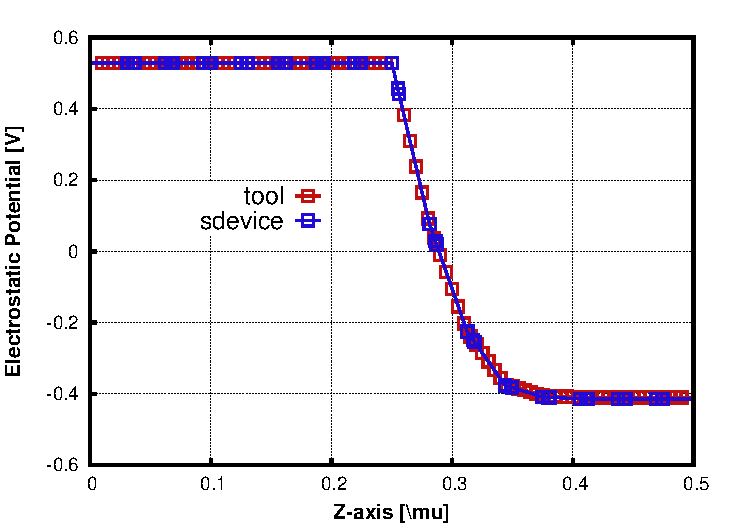
\includegraphics[scale=0.3]{N1e19_P1e17}}
	\subfigure[N20P20]
	  {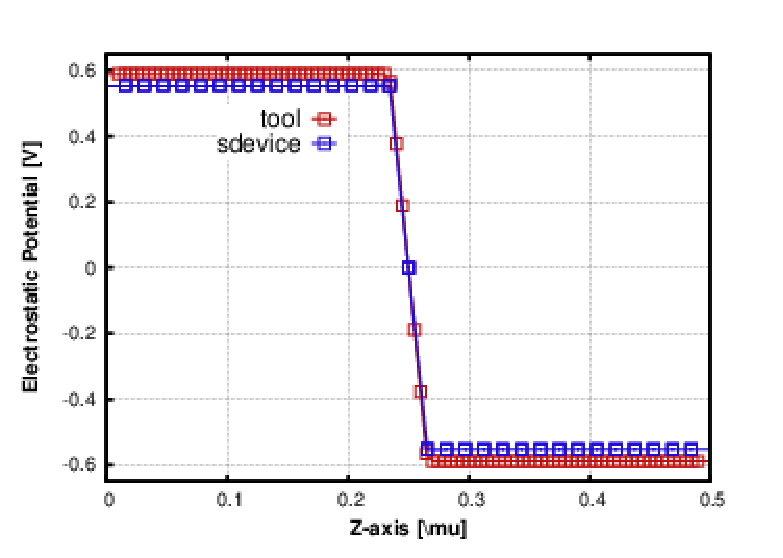
\includegraphics[scale=0.3]{N1e20_P1e20_block_POT_Z}}
\end{figure}
\end{center}
\end{column}
\begin{column}{0.5 \textwidth}
\begin{center}
\begin{figure}[!h]
         \subfigure[N20P17N19]
          {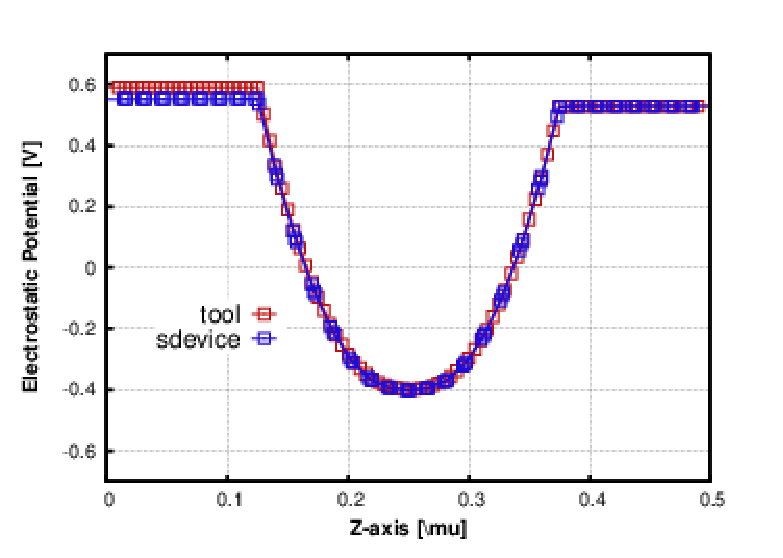
\includegraphics[scale=0.3]{N1e20_P1e17_N1e19}}
	\subfigure[N18P18]
	  {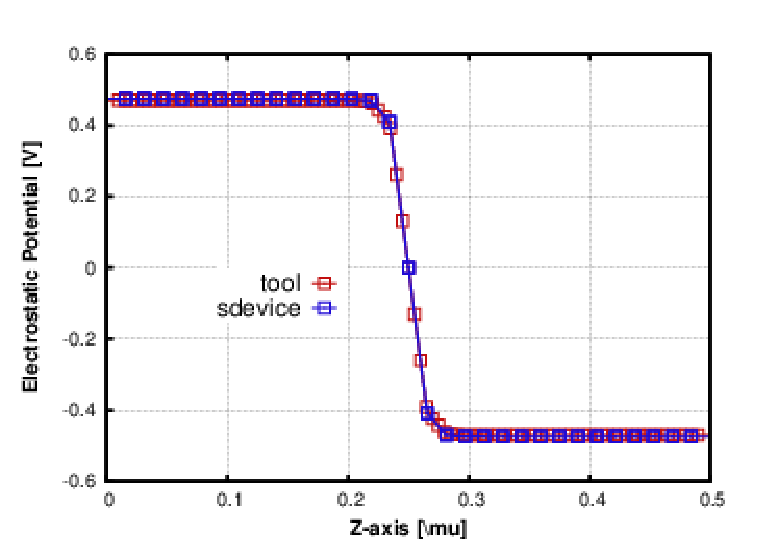
\includegraphics[scale=0.3]{N1e18_P1e18_block_POT}}
\end{figure}
\end{center}
\end{column}
\end{columns}

\end{frame}

\begin{frame}
\frametitle{Free charge plot asse Z \& Newton method (start-end)}
L'accordo si mantiene ottimo al variare della mesh (abbiamo prodotto i test lavorando con mesh fra i 450 a 70.000 nodi). Effettuando tagli ortogonali all'asse Z l'accordo si mantiene ottimo.

\begin{columns}

\begin{column}{0.5 \textwidth}
\begin{figure}[!h]
\subfigure[N18P18]
	  {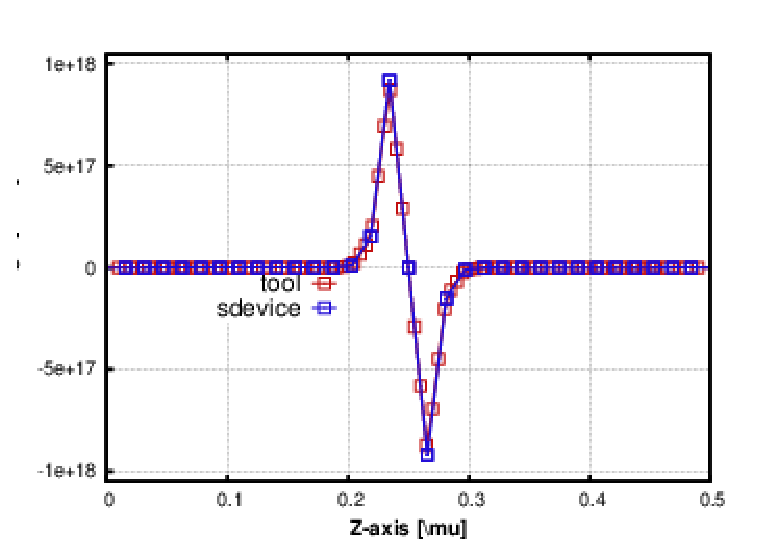
\includegraphics[scale=0.3]{N1e18_P1e18_block_CHARGE}}
	  \end{figure}
\end{column}

\begin{column}{0.5 \textwidth}
\begin{figure}[!h]
	  \subfigure[N20P20]
	  {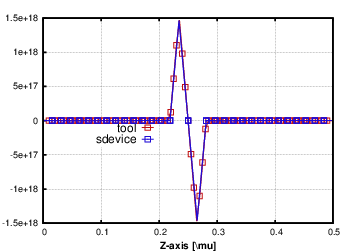
\includegraphics[scale=0.3]{N1e20_P1e20_block_CHARGE_Z}}
	  \end{figure}
\end{column}

\end{columns}

\end{frame}

\begin{frame}
\frametitle{Newton method (start-end) \& Band Diagram}
Per la visualizzazione il livello 0 \`e il vuoto, mentre la risoluzione viene calcolata mettendo a 0 il potenziale di fermi.
\begin{columns}

\begin{column}{0.25 \textwidth}
\begin{center}
\begin{figure}[!h]
          {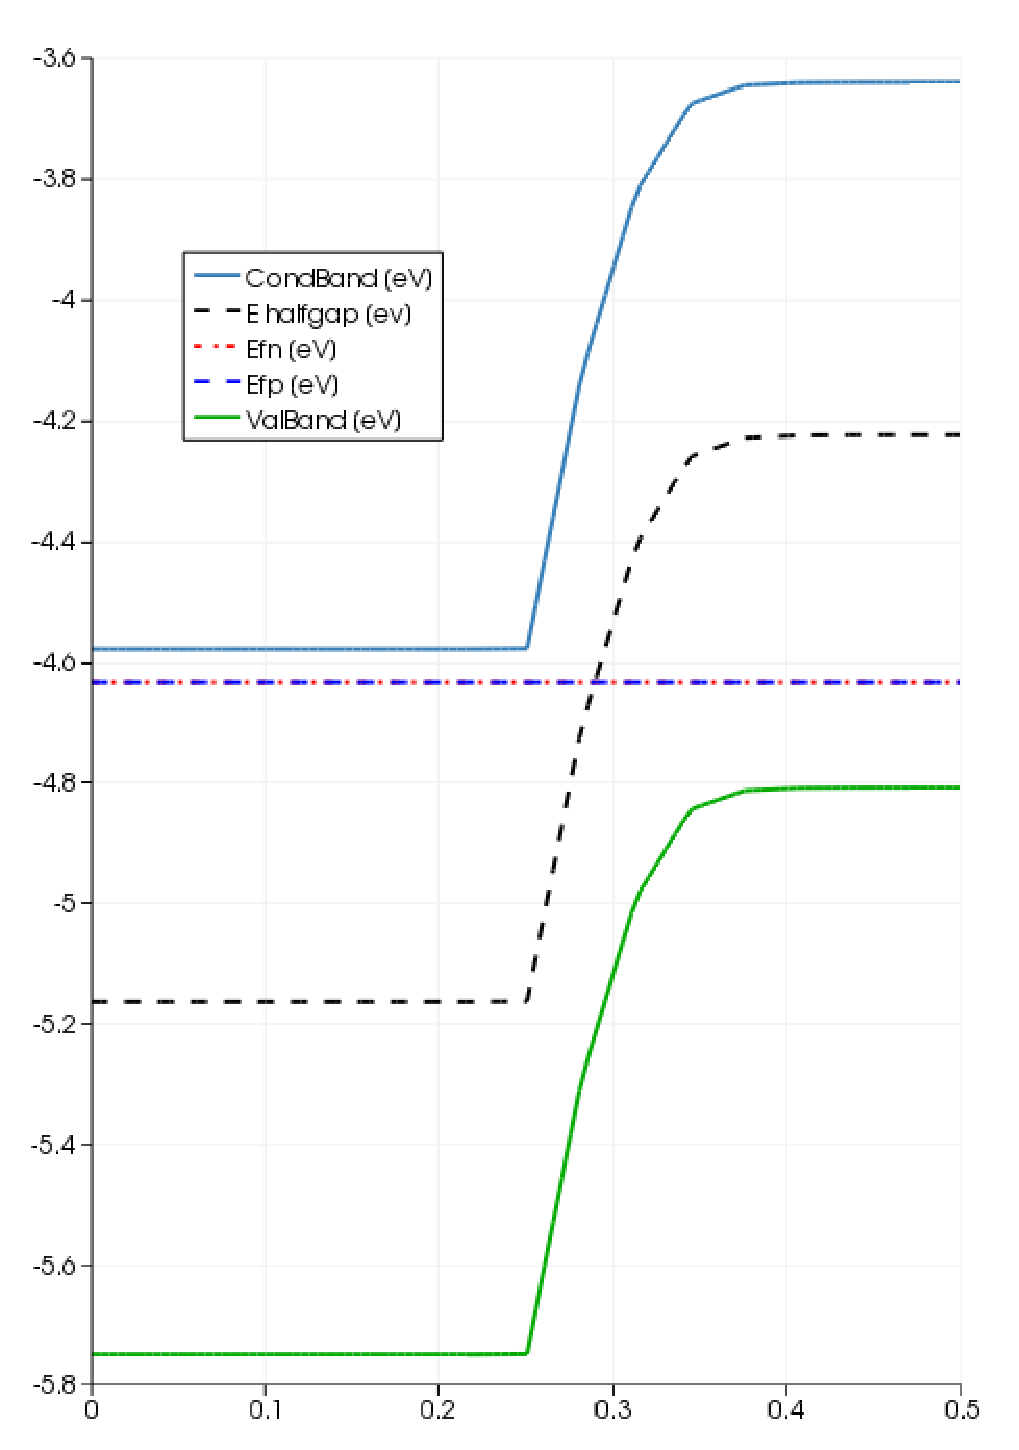
\includegraphics[scale=0.18]{N1e19_P1e17_BandDiagram}}
\end{figure}
\end{center}
\end{column}

\begin{column}{0.25 \textwidth}
\begin{center}
\begin{figure}[!h]
          {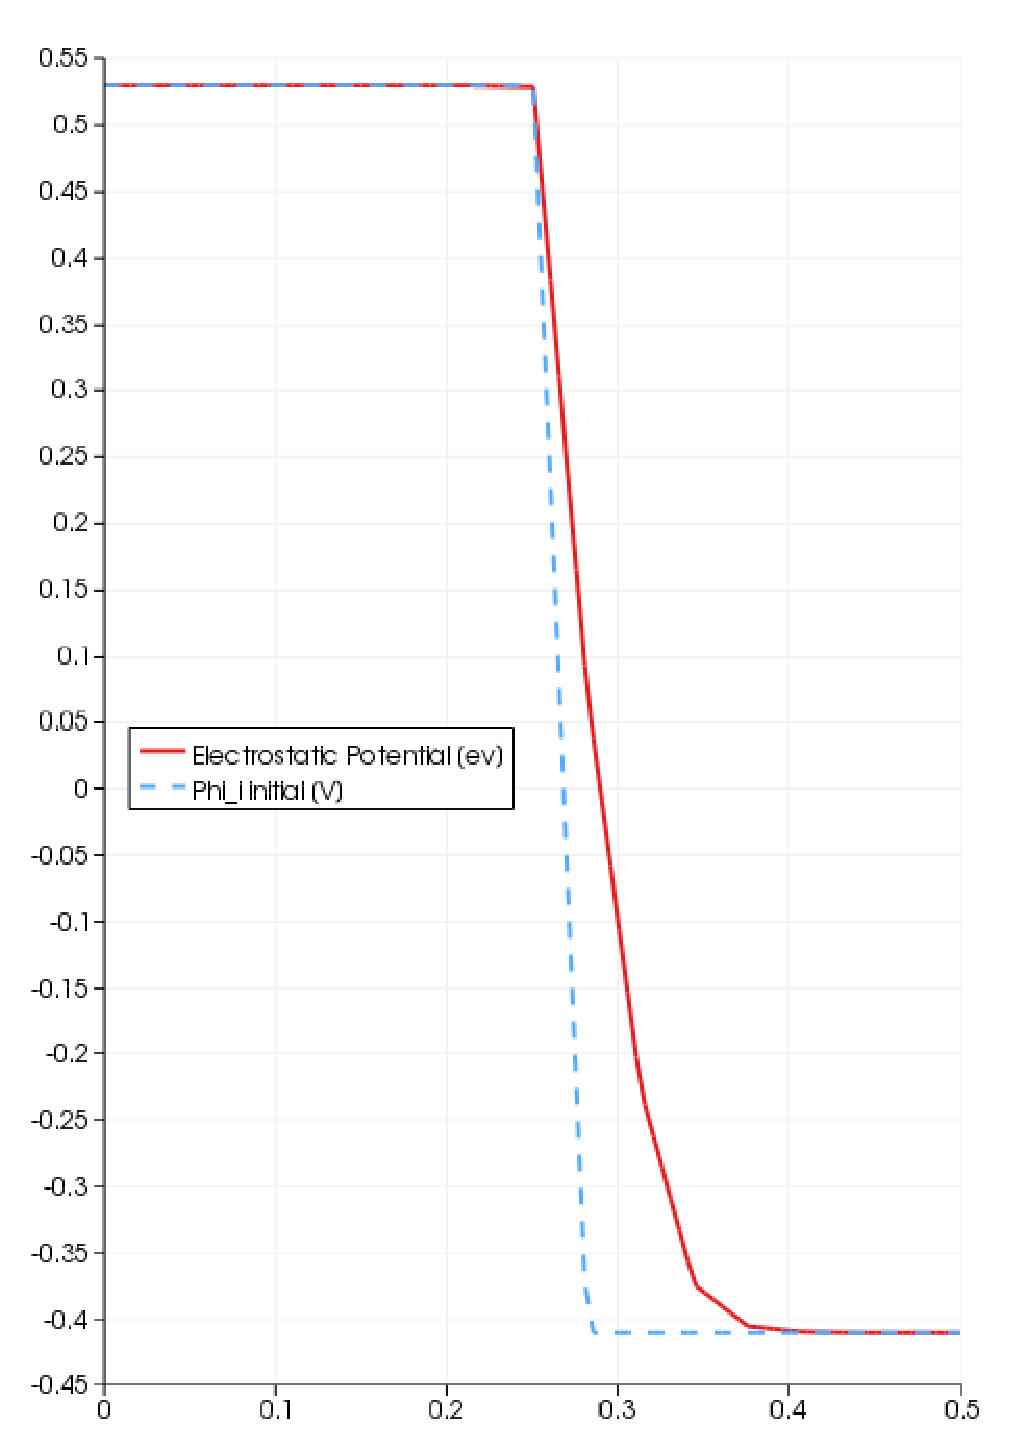
\includegraphics[scale=0.18]{N1e19_P1e17_ElectrostaticPotential}}	
\end{figure}
\end{center}
\end{column}

\begin{column}{0.25 \textwidth}
\begin{center}
\begin{figure}[!h]

          {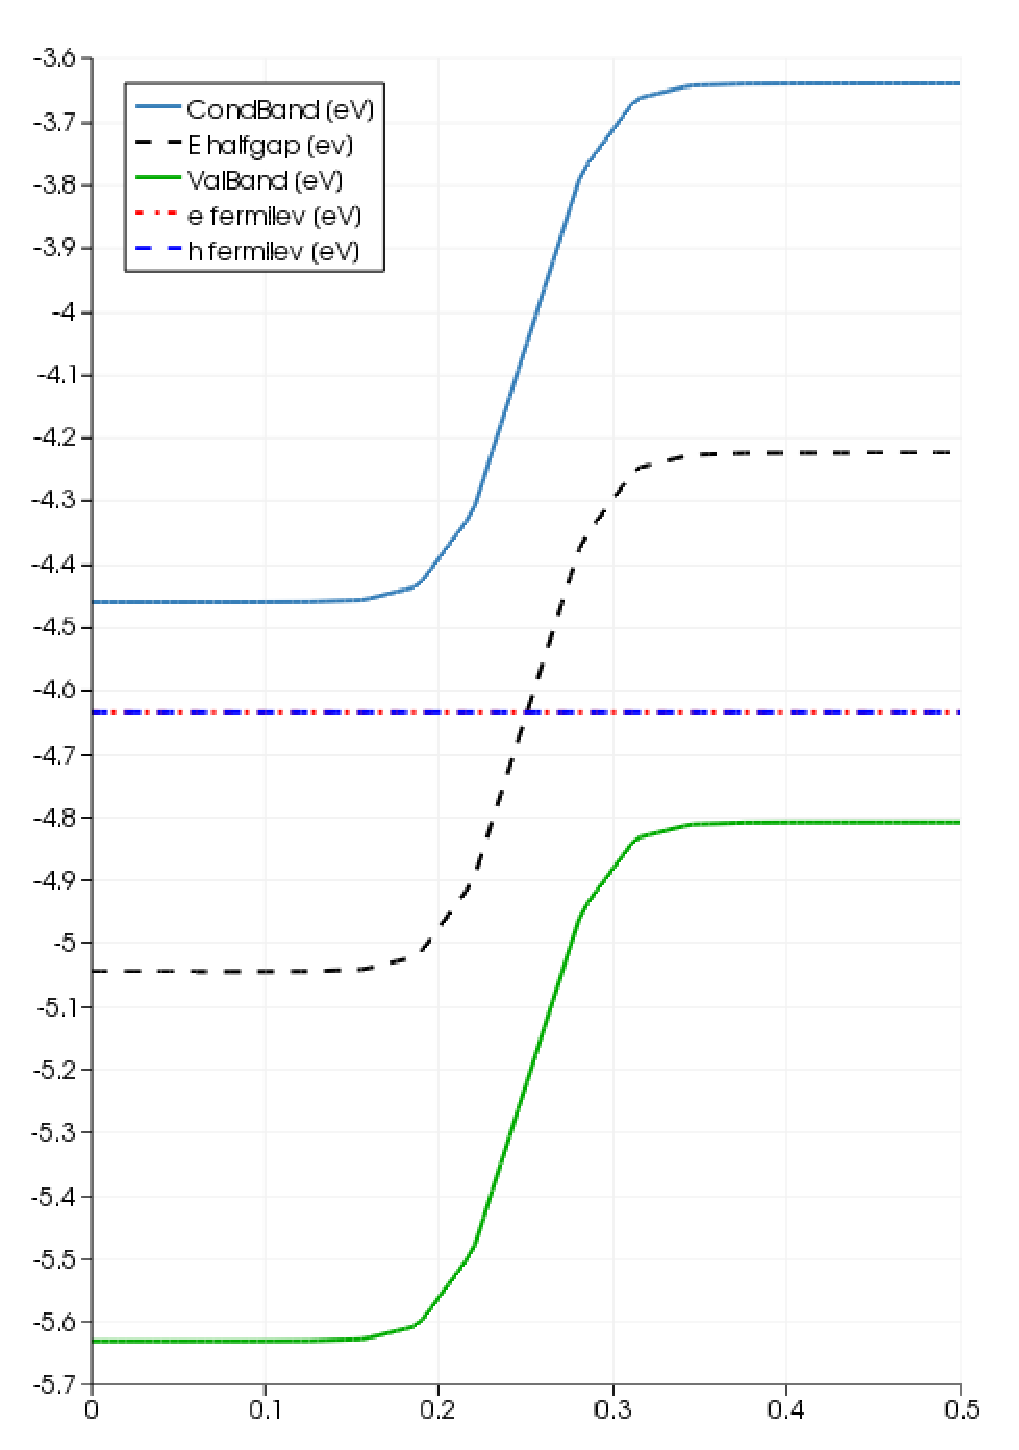
\includegraphics[scale=0.18]{N1e17_P1e17_BandDiagram}}
 \end{figure}
 \end{center}
 \end{column}
 
\begin{column}{0.25 \textwidth}
\begin{center}
\begin{figure}[!h]
          {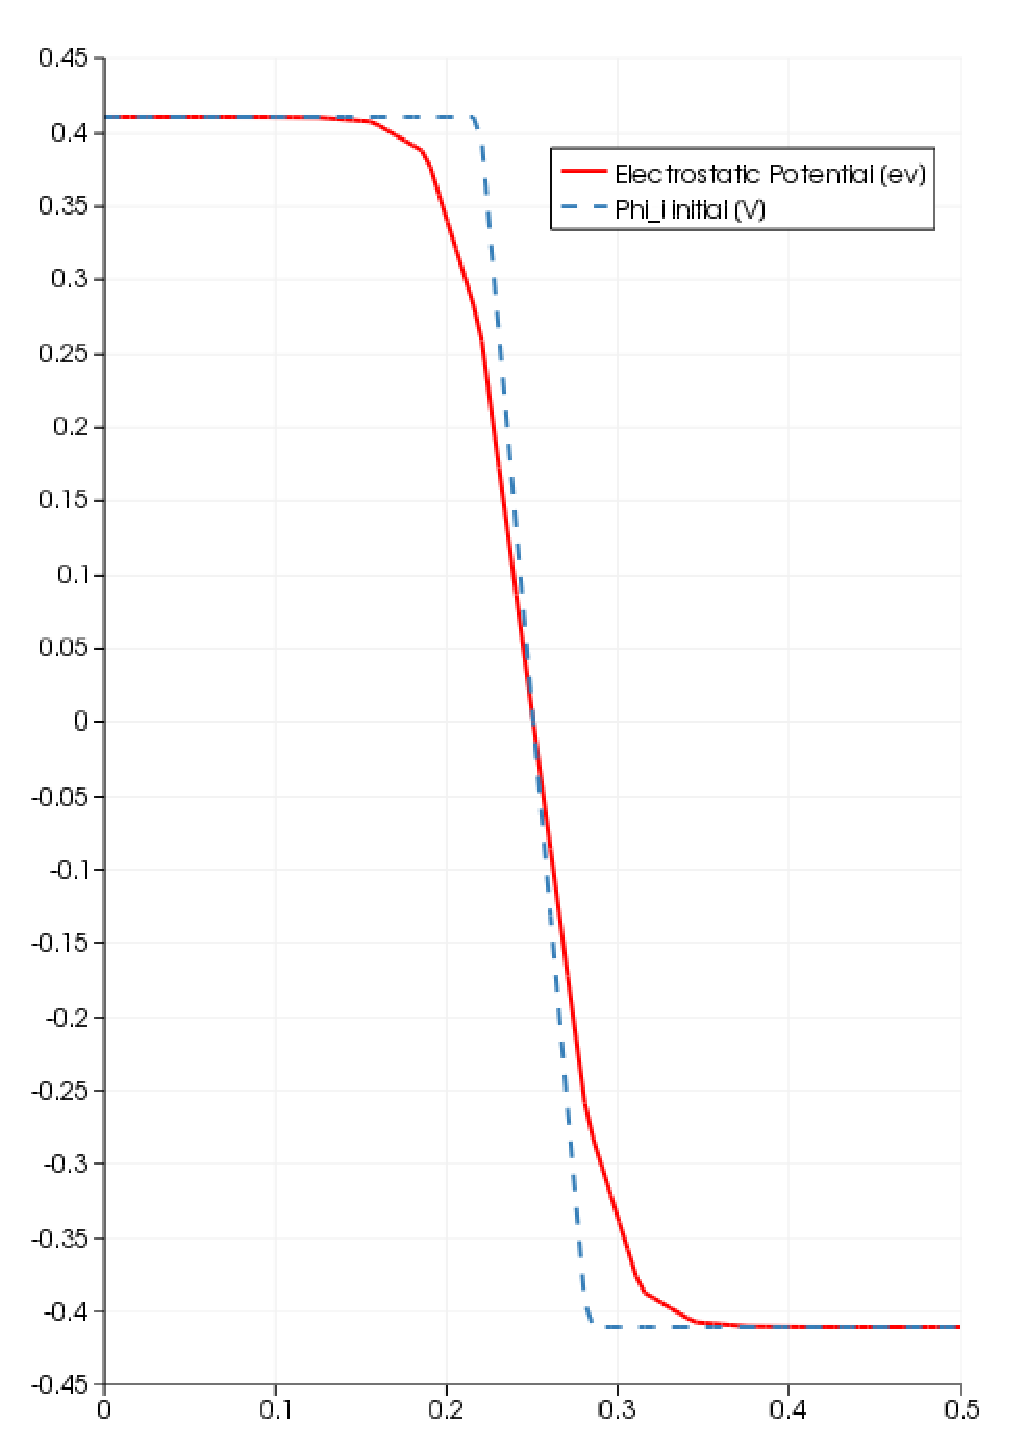
\includegraphics[scale=0.18]{N1e17_P1e17_ElectrostaticPotential}}	
\end{figure}
\end{center}
\end{column}

\end{columns}

\end{frame}





\subsection{Damping}
\begin{frame}
\tableofcontents[currentsection]
\end{frame}

\begin{frame}
\frametitle{Algoritmo implementato}
\begin{center}
Abbiamo adoperato un'oppurtuna normalizzazione del termine forzante poich\'e non usiamo variabili scalate (ordine del drogaggio)
\begin{equation*}
\begin{array}{l}
F_k = F(\varphi_k) \quad F_{k+1}=F(\varphi_k+t_k^{(j)}\delta\varphi_k) 
 \\  
t_k^{(j)}=\frac{1}{1+K_k^{(j)}\parallel F_k\parallel}  
\quad \longrightarrow \quad \parallel F_k\parallel \approx 10^{18}\Longrightarrow t_k^{(j)} \approx 0
\\  
N\approx 10^{18} \quad \tilde{t}_k^{(j)}=\frac{1}{1+K_k^{(j)}\parallel F_k\parallel_\infty N^{-1}}  
\\ 
K_k^{(j)} \quad t.c. \quad
1-\frac{\parallel F_{k+1}^{(j)} \parallel_\infty}{  \parallel F_{k} \parallel_\infty }< \delta \tilde{t}_k^{(j)} \quad\quad K_k^{(j)} = K_{base}^j
\end{array}
\end{equation*}
\begin{alertblock}{Problema}
La condizione di uscita non viene mai soddisfatta, si esce dal ciclo solo perch\`e viene opportunamente settato il maxit su $j$ (altrimenti $t_k^{(j)}\rightarrow 0$ e il sistema non evolve).
\end{alertblock}
\end{center}
\end{frame}

\begin{frame}
\frametitle{Andamento del residuo}
Comportamenti differenti del residuo sulla risoluzione di Newton senza damping al variare dei drogaggi.
\begin{center}
\begin{figure}[!h]
          {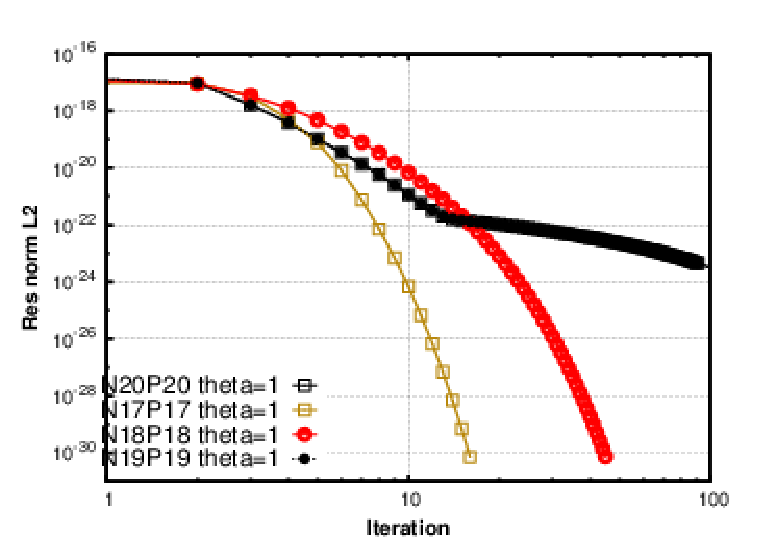
\includegraphics[scale=0.6]{Cfr_Doping}}

\end{figure}
\end{center}


\end{frame}

\begin{frame}
\frametitle{Damping}
\begin{columns}
\begin{column}{0.5 \textwidth}
\begin{exampleblock}{Parametri settati da input file}
\begin{itemize}
\item[-] $K_{base}$
\item[-] $\delta$
\item[-] N (fattore di normalizzazione)
\end{itemize}
\end{exampleblock}
\end{column}
\begin{column}{0.4 \textwidth}
$NOTA:$ abbiamo usato il caso N20P20 pi\`u lento a convergere
\end{column}
\end{columns}
\begin{center}
\begin{figure}[!h]
          {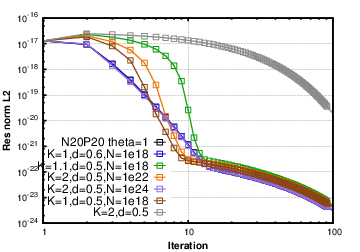
\includegraphics[scale=0.58]{Cfr_DAMPING}}
\end{figure}
\end{center}
\end{frame}




\section{Oxide}
\begin{frame}
\tableofcontents[currentsection]
\end{frame}

\begin{frame}
\frametitle{Esperimento ossido}
\begin{columns}
\begin{column}{0.5 \textwidth}
Abbiamo testato il risolutore lineare in due differenti situazioni, confrontate entrambe con sdevice. 

Per prima vediamo il caso $L_{contatto} = L_{lato}$
\end{column}
\begin{column}{0.5 \textwidth}
\begin{center}
\begin{figure}[!h]
          {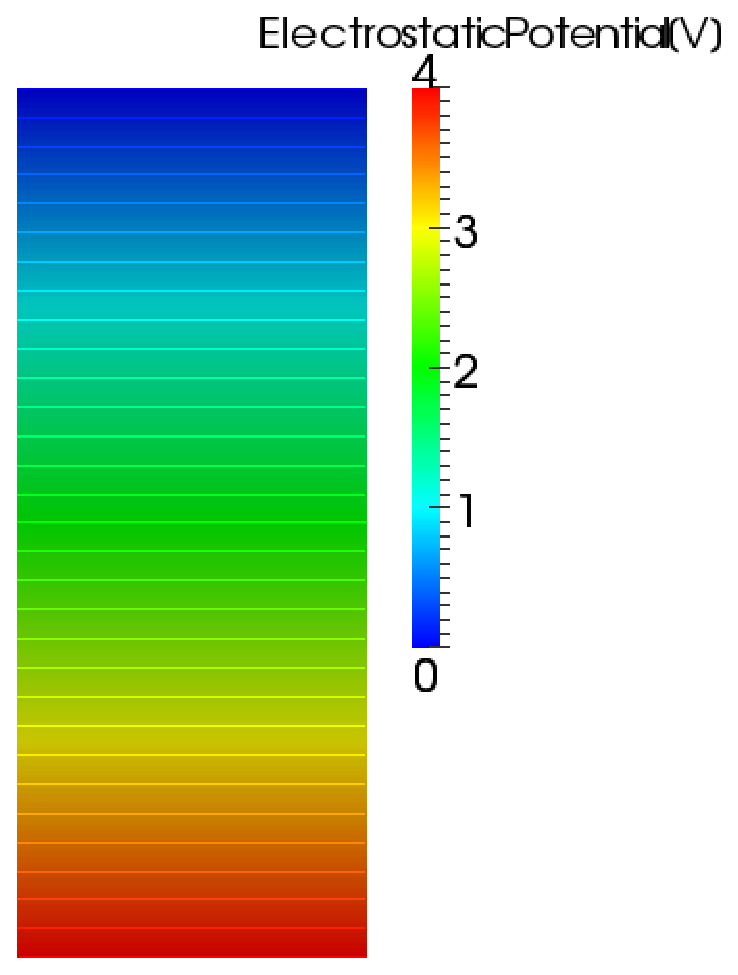
\includegraphics[scale=0.3]{ossidolineare}}
          \end{figure}
\end{center}
\end{column}

\end{columns}


\end{frame}

\begin{frame}
\frametitle{Esperimento ossido}
Di seguito il caso $L_{contatto} < L_{lato}$, soluzione non lineare

\begin{columns}

\begin{column}{0.3 \textwidth}
\begin{center}
\begin{figure}[!h]
          {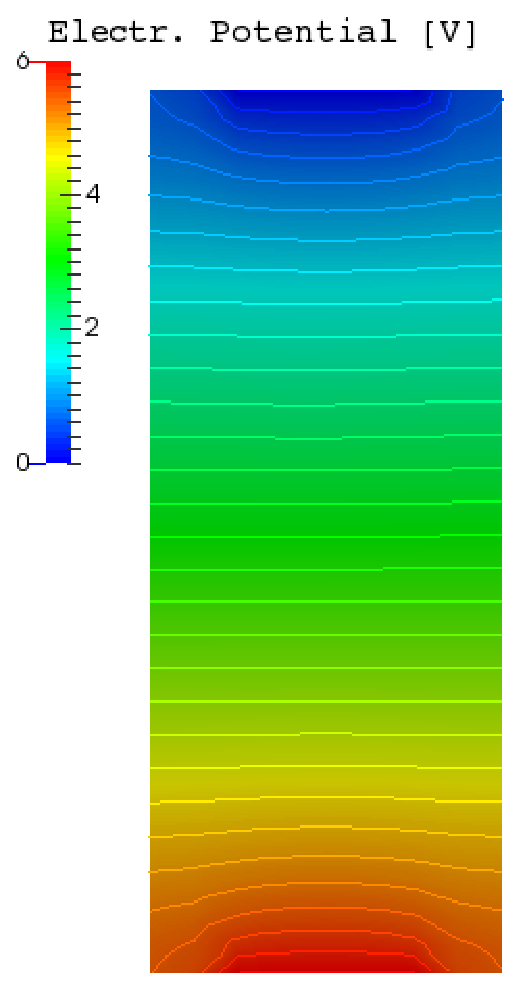
\includegraphics[scale=0.3]{potential}}
          \end{figure}
\end{center}
\end{column}

\begin{column}{0.3 \textwidth}
\begin{center}
\begin{figure}[!h]
          {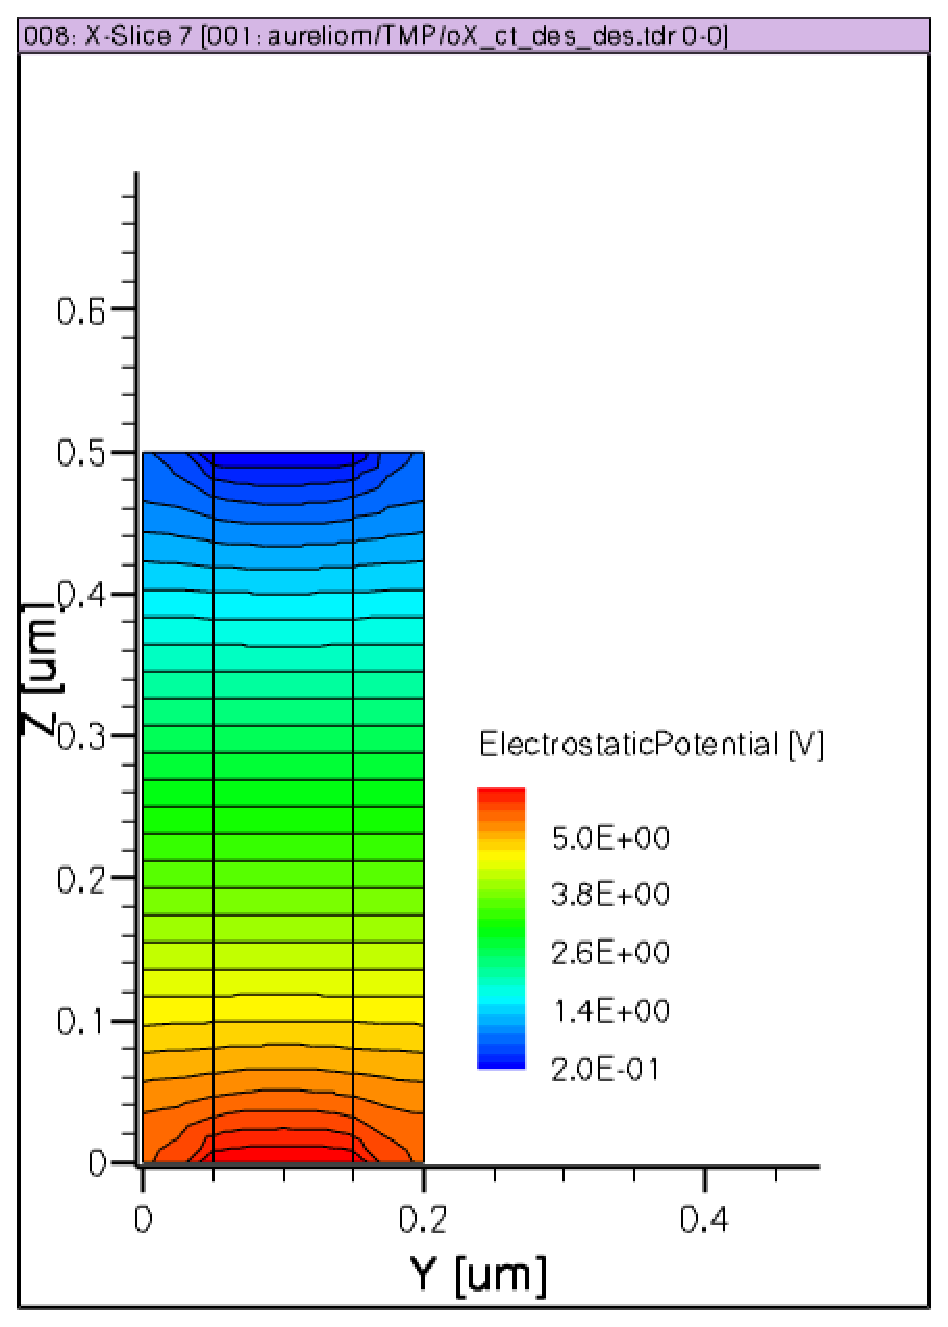
\includegraphics[scale=0.3]{ossido}}
          \end{figure}
\end{center}
\end{column}

\end{columns}

\end{frame}



\section{Silicon in oxide}

\begin{frame}
\tableofcontents[currentsection]
\end{frame}

\begin{frame}
\frametitle{Formulazione problema}

\begin{columns}
\begin{column}{0.5\textwidth}
\begin{equation*}
\begin{cases}
\nabla \cdot ( -\epsilon_0 \epsilon_r \nabla \varphi) = q(p-n+D) & \text{in $\Omega_{Si}$}\\
\nabla \cdot ( -\epsilon_0 \epsilon_r \nabla \varphi) = 0 & \text{in $\Omega_{Ox}$}\\
\nabla \varphi \cdot \vect{n} =0 & \text{su $\Gamma_{Ox}$ }\\
\varphi = \varphi_K & \text{su $\Gamma_{K}$}\\
\varphi = \varphi_A & \text{su $\Gamma_{A}$}\\
\end{cases}
\end{equation*}
\end{column}
\end{columns}

\begin{center}
\begin{tikzpicture}
[scale=1.5]

\draw [thick] (2,0) rectangle (3,1);
\node at (-0.25,1.25) {$\Gamma_{A}$};
\node at (3.3,0.5) {$\Gamma_{K}$};
\node at (2,1.75) {$\Gamma_{Ox}$};
\node at (1,1) {$\Omega_{Si}$};
\node at (0.4,0.4) {$\Omega_{Ox}$};


\draw [thick] (2,1)--(0,2)--(1,2)--(3,1);
\draw [thick] (2,0)--(0,1)--(0,2);

%\draw [dashed,thick] (0,1)--(1,1)--(1,2);
%\draw [dashed,thick] (1,1)--(3,0);

\draw [pattern=north west lines, pattern color=gray, thick] (2.1,0.1) rectangle (2.9,0.9);


\draw [dashed] (0.1,1.1) rectangle (0.9,1.9);
\draw [dashed] (2.9,0.1)--(0.9,1.1);
\draw [dashed] (2.9,0.9)--(0.9,1.9);
\draw [dashed] (2.1,0.1)--(0.1,1.1);
\draw [dashed] (2.1,0.9)--(0.1,1.9);
%\draw [thick,dashed] (2.9,0.1)--(0.9,1.1);

\end{tikzpicture}

\end{center}
\end{frame}

\begin{frame}
\frametitle{Newton}

\begin{equation*}
\begin{cases}
-\nabla \cdot ( \epsilon_{Si} \nabla \delta\varphi) + \sigma\delta\varphi = \nabla \cdot ( \epsilon_{Si} \nabla \varphi) + q(p-n+D) & \text{in $\Omega_{Si}$}\\
-\nabla \cdot ( \epsilon_{Ox} \nabla \delta\varphi) = \nabla \cdot ( \epsilon_{Ox} \nabla \varphi) & \text{in $\Omega_{Ox}$}\\
\nabla \delta\varphi \cdot \vect{n} =0 & \text{su $\Gamma_{Ox}$ }\\
\delta\varphi = 0 & \text{su $\Gamma_{K}$}\\
\delta\varphi = 0 & \text{su $\Gamma_{A}$}\\
\end{cases}
\end{equation*}

\begin{alertblock}{Domanda:}
Cosa bisogna imporre, come valore di forzante e coefficiente di reazione, sui nodi di frontiera fra il bulk di silicio e l'ossido?
\end{alertblock}

\end{frame}


\begin{frame}
\frametitle{Sezioni fissate le coordinate X e Z}
\begin{columns}
\begin{column}{0.5 \textwidth}
\begin{center}
Valori al bordo pari al silicio
\begin{figure}[!h]
         \subfigure[Potenziale]
          {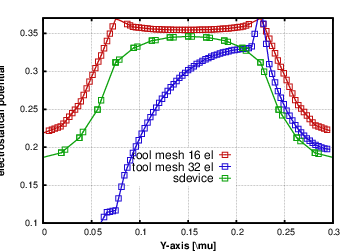
\includegraphics[scale=0.3]{N1e17_P1e17_OX_electro_lineZ002_withsigma}}
	\subfigure[Carica]
	  {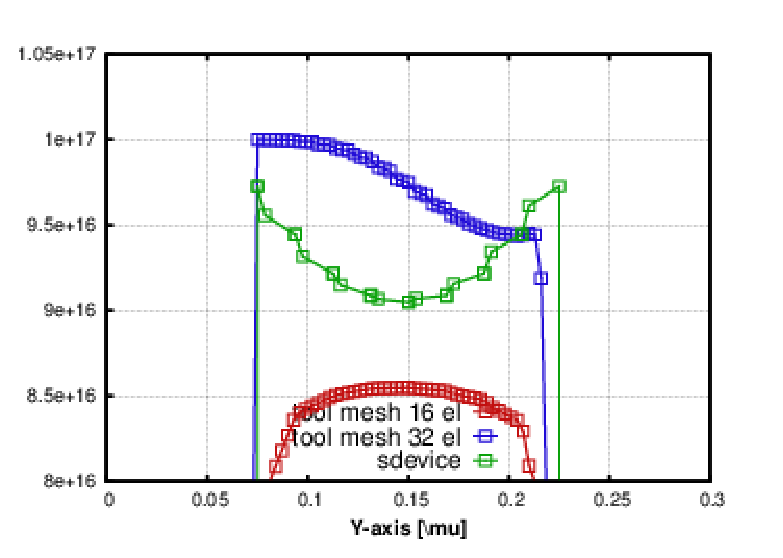
\includegraphics[scale=0.3]{N1e17_P1e17_OX_spacecharge_lineZ002_withsigma}}
\end{figure}
\end{center}
\end{column}
\begin{column}{0.5 \textwidth}
\begin{center}
Valori al bordo pari all'ossido
\begin{figure}[!h]
         \subfigure[Potenziale]
          {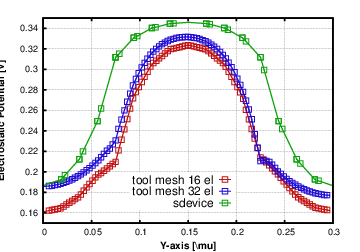
\includegraphics[scale=0.3]{N1e17_P1e17_OX_lineZ002}}
	\subfigure[Carica]
	  {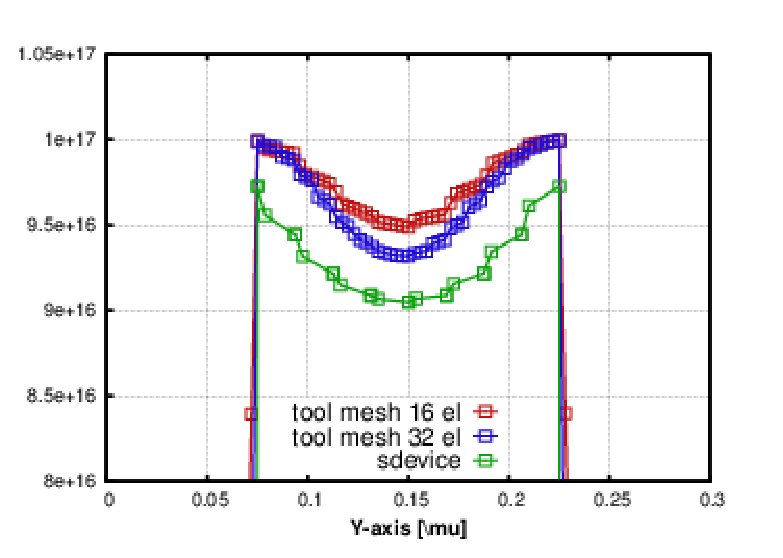
\includegraphics[scale=0.3]{N1e17_P1e17_OX_spacecharge_lineZ002}}
\end{figure}
\end{center}
\end{column}
\end{columns}

\end{frame}


\begin{frame}
\frametitle{Decisione empirica}
\begin{itemize}
\item[1.] Le soluzioni non coincidono pi\`u con sdevice
\item[2.] La scelta di imporre i valori relativi all'ossido sembra portare la soluzione pi\`u vicina ad sdevice 
\end{itemize}
Nei test successivi adottiamo la scelta di valori pari all'ossido sull'interfaccia.
\end{frame}

\subsection{N16P16}
\begin{frame}
\tableofcontents[currentsection]
\end{frame}

\begin{frame}
\frametitle{Asimmetria-Potenziale N16P16}
Evidente asimmetria fra le differenti sezioni e problema allineamento valore di interfaccia sulla frontiera ossido silicio.
\begin{columns}

\begin{column}{0.3 \textwidth}
\begin{center}
\begin{figure}[!h]
         \subfigure[Sezione XZ]
          {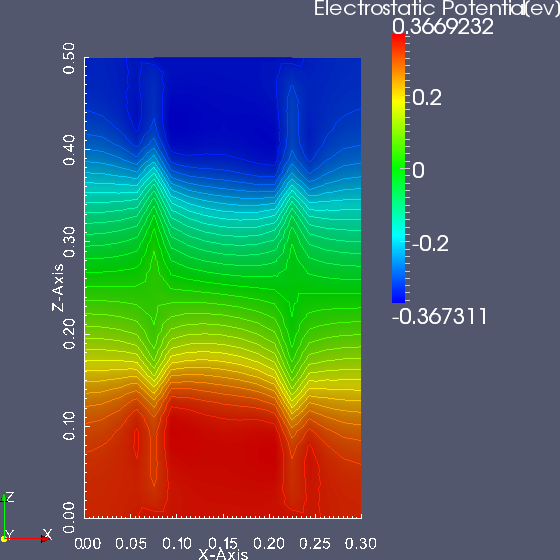
\includegraphics[scale=0.18]{N16P16OX_POT_tool_XZ}}
          \end{figure}
\end{center}
\end{column}

\begin{column}{0.3 \textwidth}
\begin{center}
\begin{figure}[!h]
         \subfigure[Sezione YZ]
          {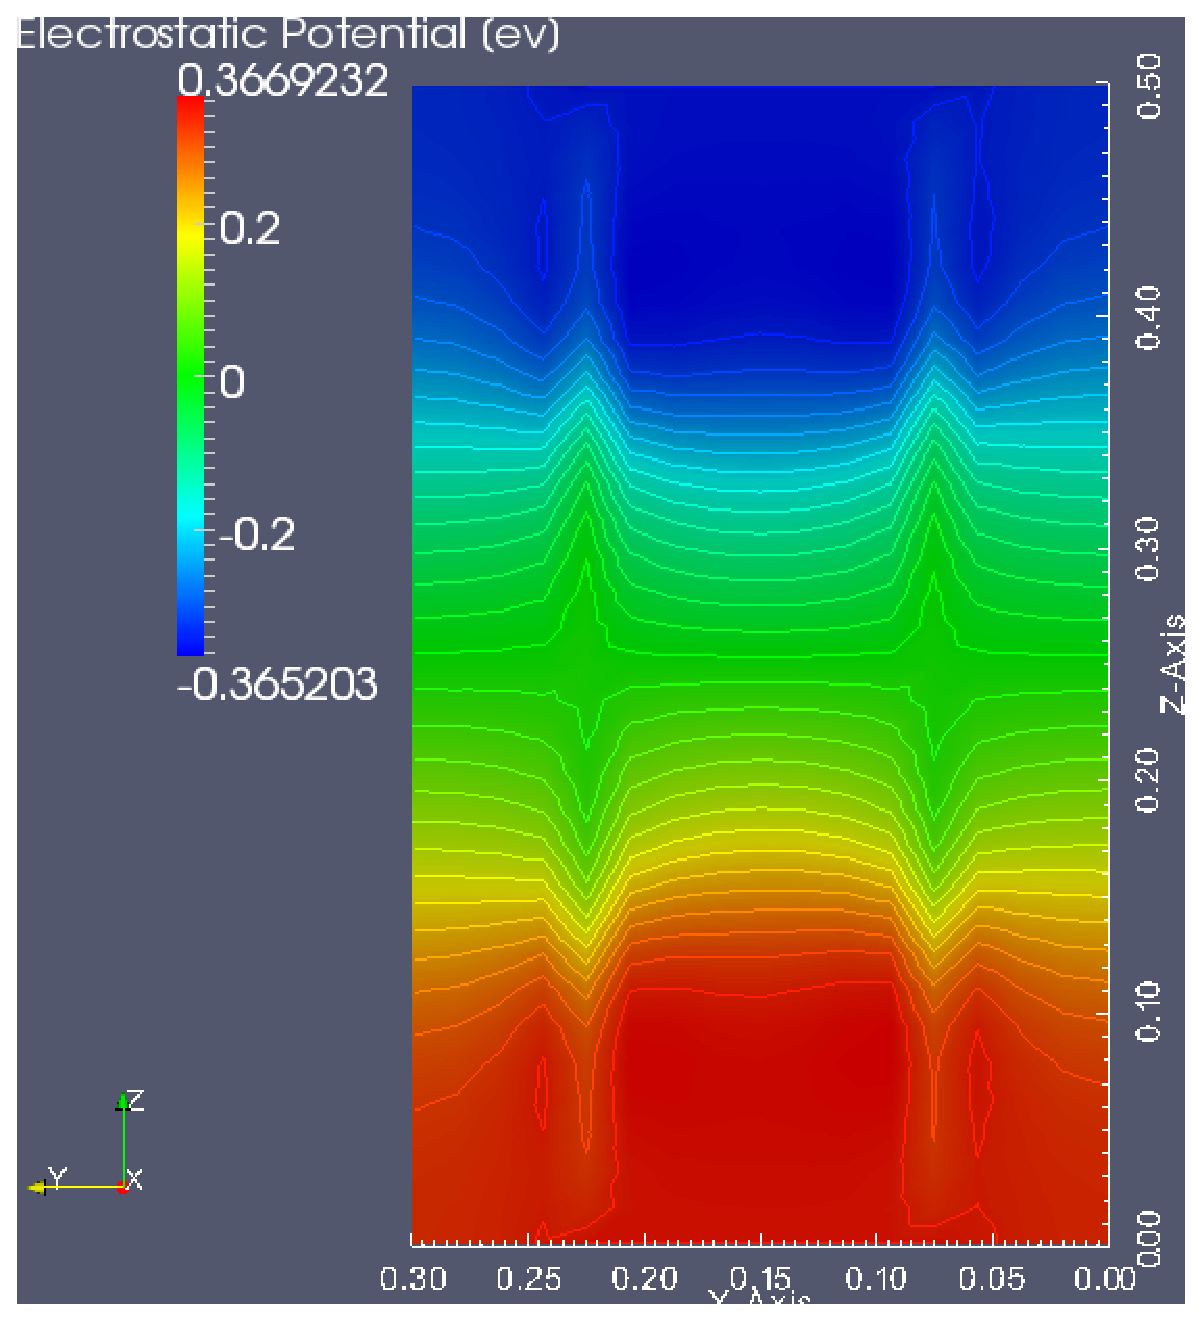
\includegraphics[scale=0.18]{N16P16OX_POT_tool_YZ}}
\end{figure}
\end{center}
\end{column}

\begin{column}{0.3 \textwidth}
\begin{center}
\begin{figure}[!h]
         \subfigure[Sdevice]
          {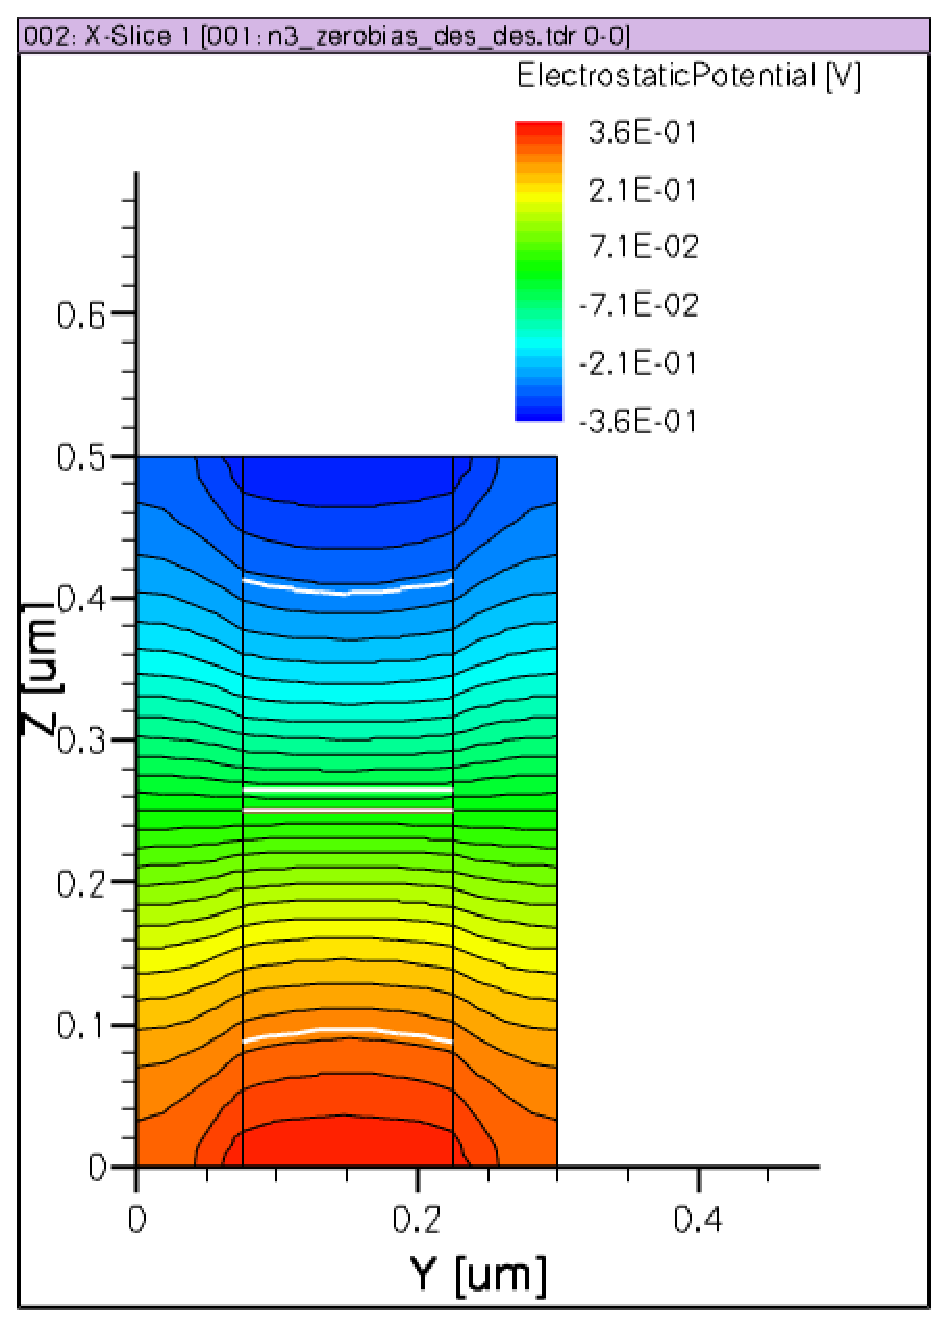
\includegraphics[scale=0.18]{N16P16OX_POT_sdevice_YZ}}
\end{figure}
\end{center}
\end{column}

\end{columns}

\end{frame}



\begin{frame}
\frametitle{Picchi inaspettati - Free Charge N16P16}
Valori numerici nella prima parte di zona svuotata soddisfacienti. Cambiamento di tendenza avvicinandosi ai contatti. Instabilit\`a?Condizioni di bordo applicate male?
\begin{columns}

\begin{column}{0.5 \textwidth}
\begin{center}
\begin{figure}[!h]
          {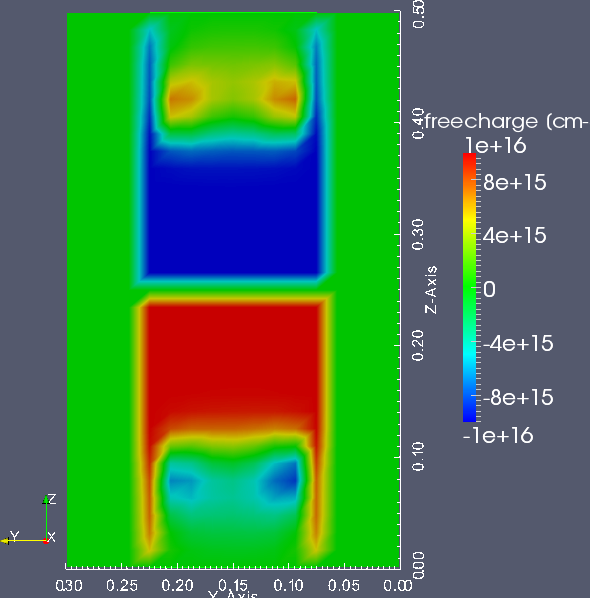
\includegraphics[scale=0.25]{N16P16OX_Q_tool_YZ}}
          \end{figure}
\end{center}
\end{column}

\begin{column}{0.5 \textwidth}
\begin{center}
\begin{figure}[!h]
          {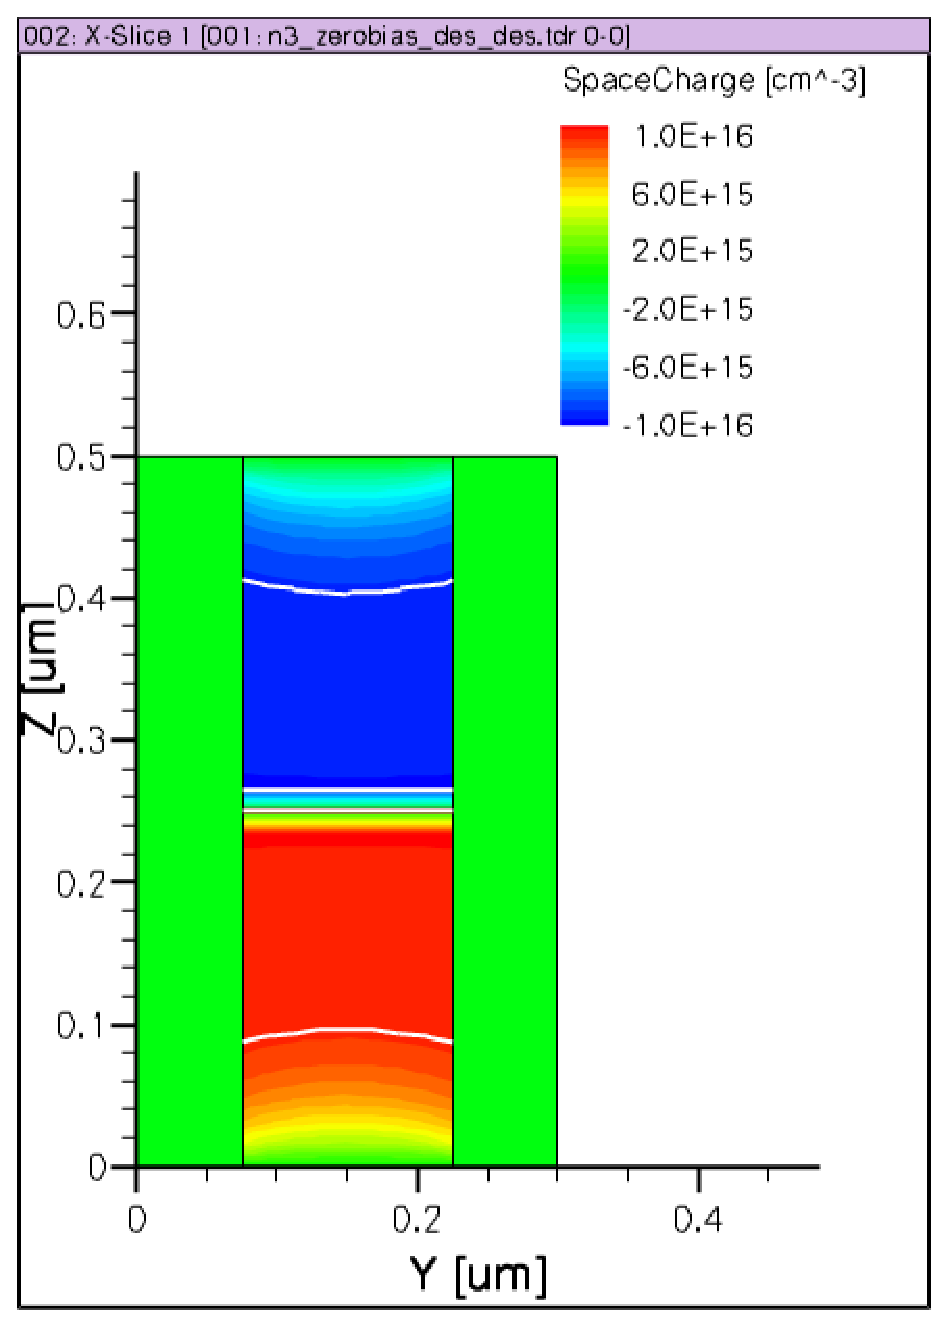
\includegraphics[scale=0.25]{N16P16OX_Q_sdevice_YZ}}
\end{figure}
\end{center}
\end{column}

\end{columns}

\end{frame}

\subsection{N17P17}
\begin{frame}
\tableofcontents[currentsection]
\end{frame}

\begin{frame}
\frametitle{Asimmetria - Potenziale N17P17}
Asimmetria accentuata (o forse prima era mascherata dai problemi di interfaccia?). Sovraddiffusione del potenziale all'interno dell'ossido.
\begin{columns}

\begin{column}{0.3 \textwidth}
\begin{center}
\begin{figure}[!h]
\subfigure[Sezione XZ]
          {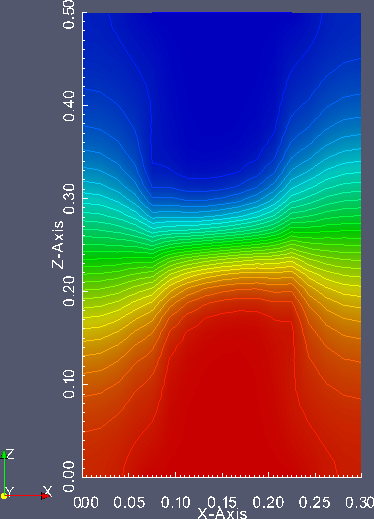
\includegraphics[scale=0.2]{N17P17OX_POT_tool_XZ}}
          \end{figure}
\end{center}
\end{column}

\begin{column}{0.3 \textwidth}
\begin{center}
\begin{figure}[!h]
\subfigure[Sezione YZ]
          {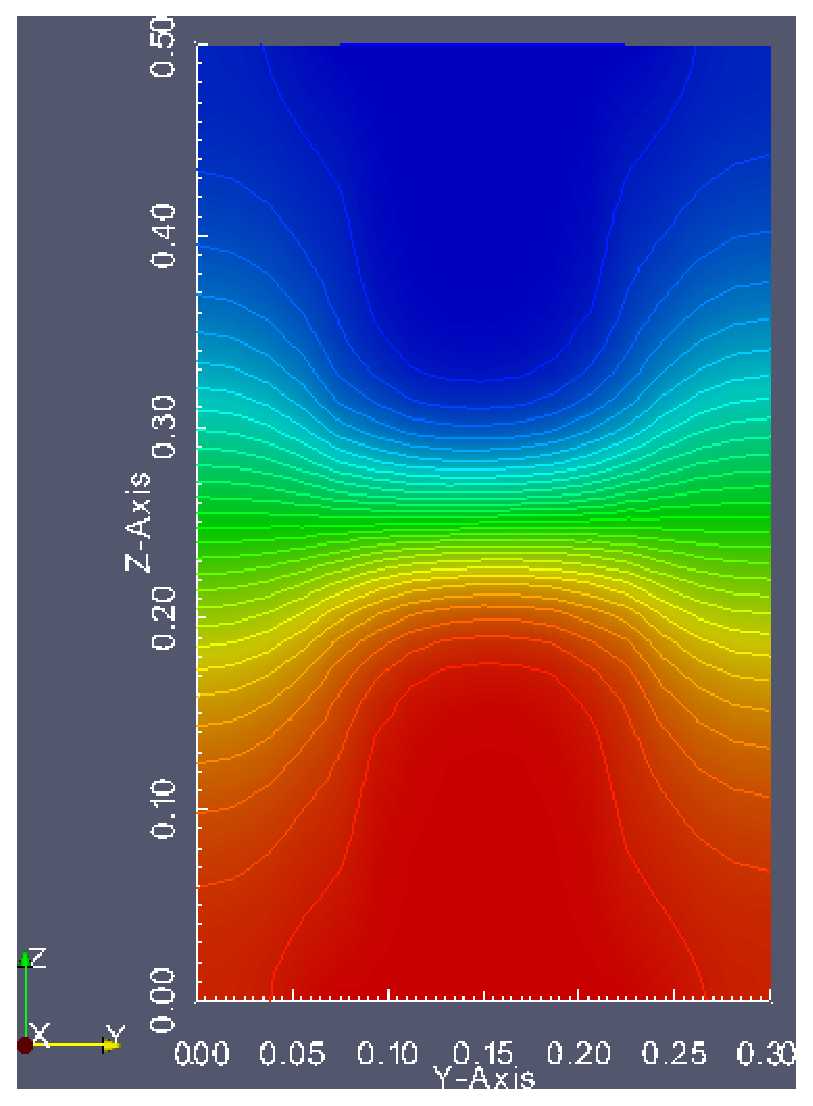
\includegraphics[scale=0.2]{N17P17OX_POT_tool_YZ}}
\end{figure}
\end{center}
\end{column}

\begin{column}{0.3 \textwidth}
\begin{center}
\begin{figure}[!h]
\subfigure[Sdevice]
          {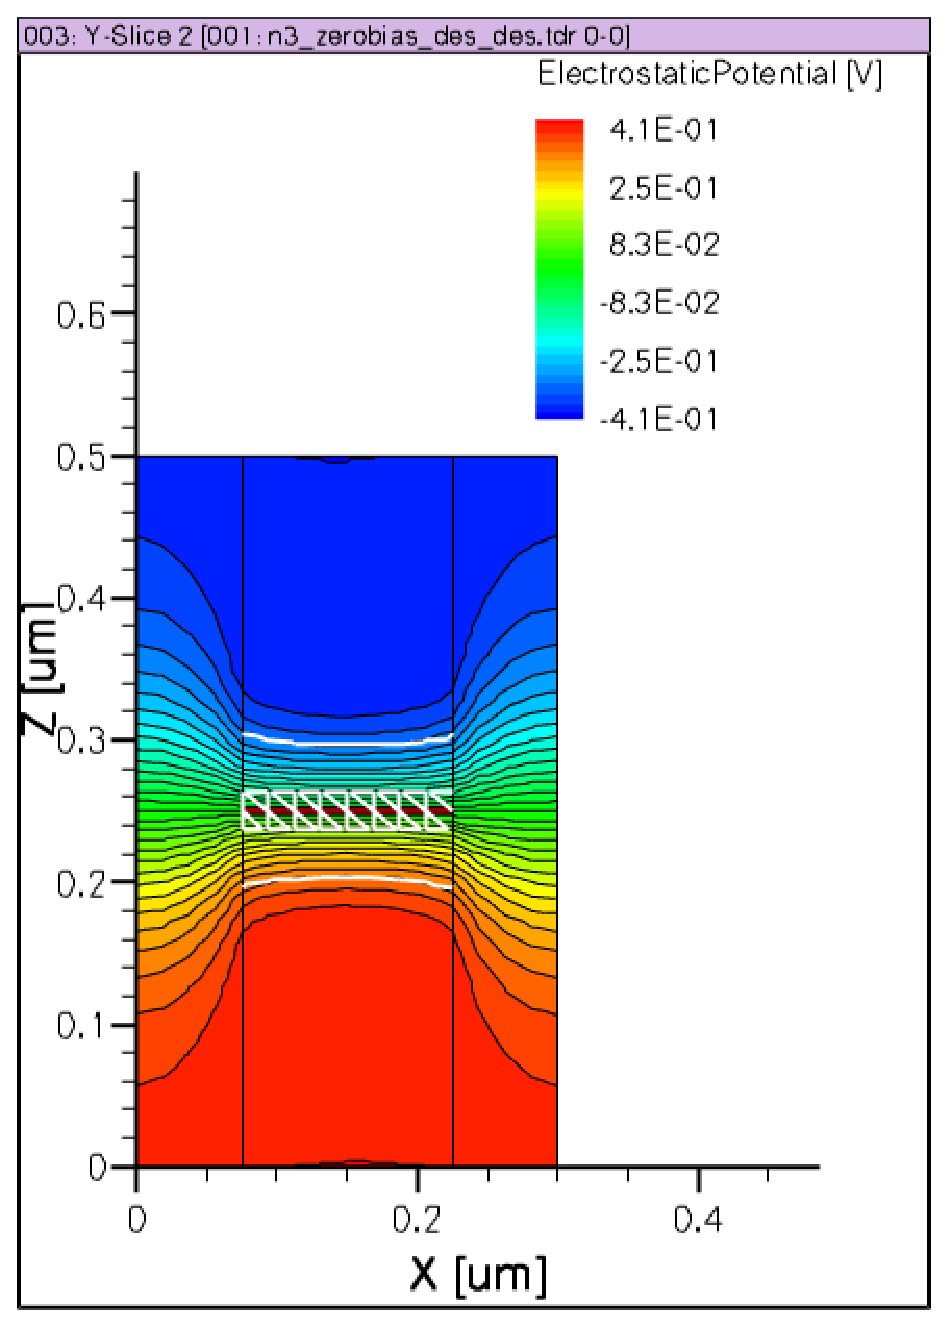
\includegraphics[scale=0.2]{N17P17OX_sdevice_XZ}}
\end{figure}
\end{center}
\end{column}

\end{columns}

\end{frame}




\begin{frame}
\frametitle{Asimmetria - Free Charge N17P17}
Ripercussioni della asimmetria evidenti sulla carica. Migliore grafico ottenuto per valori e distribuzione (l'apporto sovradiffusivo si fa notare allungando maggiormente le code di zona svuotata)
\begin{columns}

\begin{column}{0.3 \textwidth}
\begin{center}
\begin{figure}[!h]
\subfigure[Sezione XZ]
          {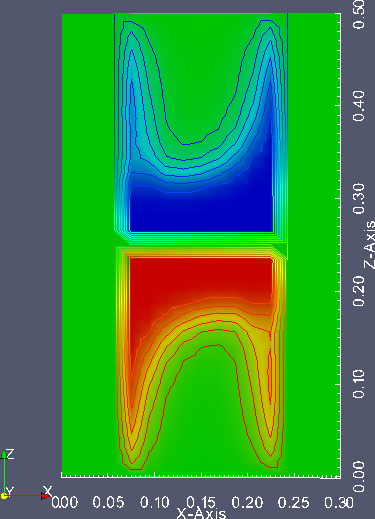
\includegraphics[scale=0.2]{N17P17OX_Q_tool_XZ}}
          \end{figure}
\end{center}
\end{column}

\begin{column}{0.3 \textwidth}
\begin{center}
\begin{figure}[!h]
\subfigure[Sezione YZ]
          {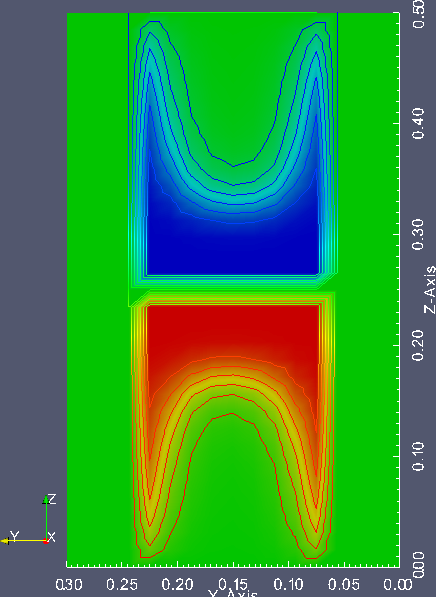
\includegraphics[scale=0.2]{N17P17OX_Q_tool_YZ}}
\end{figure}
\end{center}
\end{column}

\begin{column}{0.3 \textwidth}
\begin{center}
\begin{figure}[!h]
\subfigure[Sdevice]
          {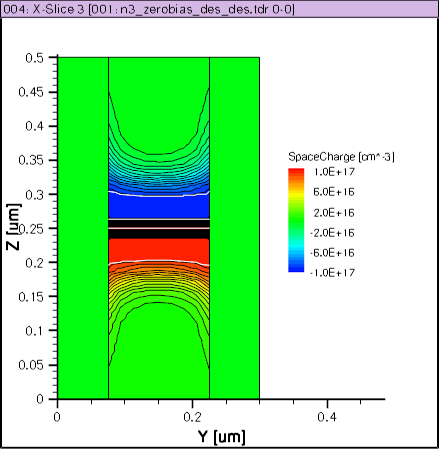
\includegraphics[scale=0.2]{N17P17OX_Q_sdevice_YZ}}
\end{figure}
\end{center}
\end{column}

\end{columns}

\end{frame}

\subsection{N19P19}
\begin{frame}
\tableofcontents[currentsection]
\end{frame}

\begin{frame}
\frametitle{Asimmetria scomparsa - Potenziale  N19P19}
Smorzamento dell'asimmetria dei risulatati, probabilmente dovuto al drogaggio alto (che rendendo pi\`u fine la zona svuotata non permette di valutare un'eventuale asimmetria). Fenomeno di sovraddiffusione contenuto (o assente?) probabilmente per la medesima motivazione.
\begin{columns}

\begin{column}{0.3 \textwidth}
\begin{center}
\begin{figure}[!h]
\subfigure[Sezione XZ]
          {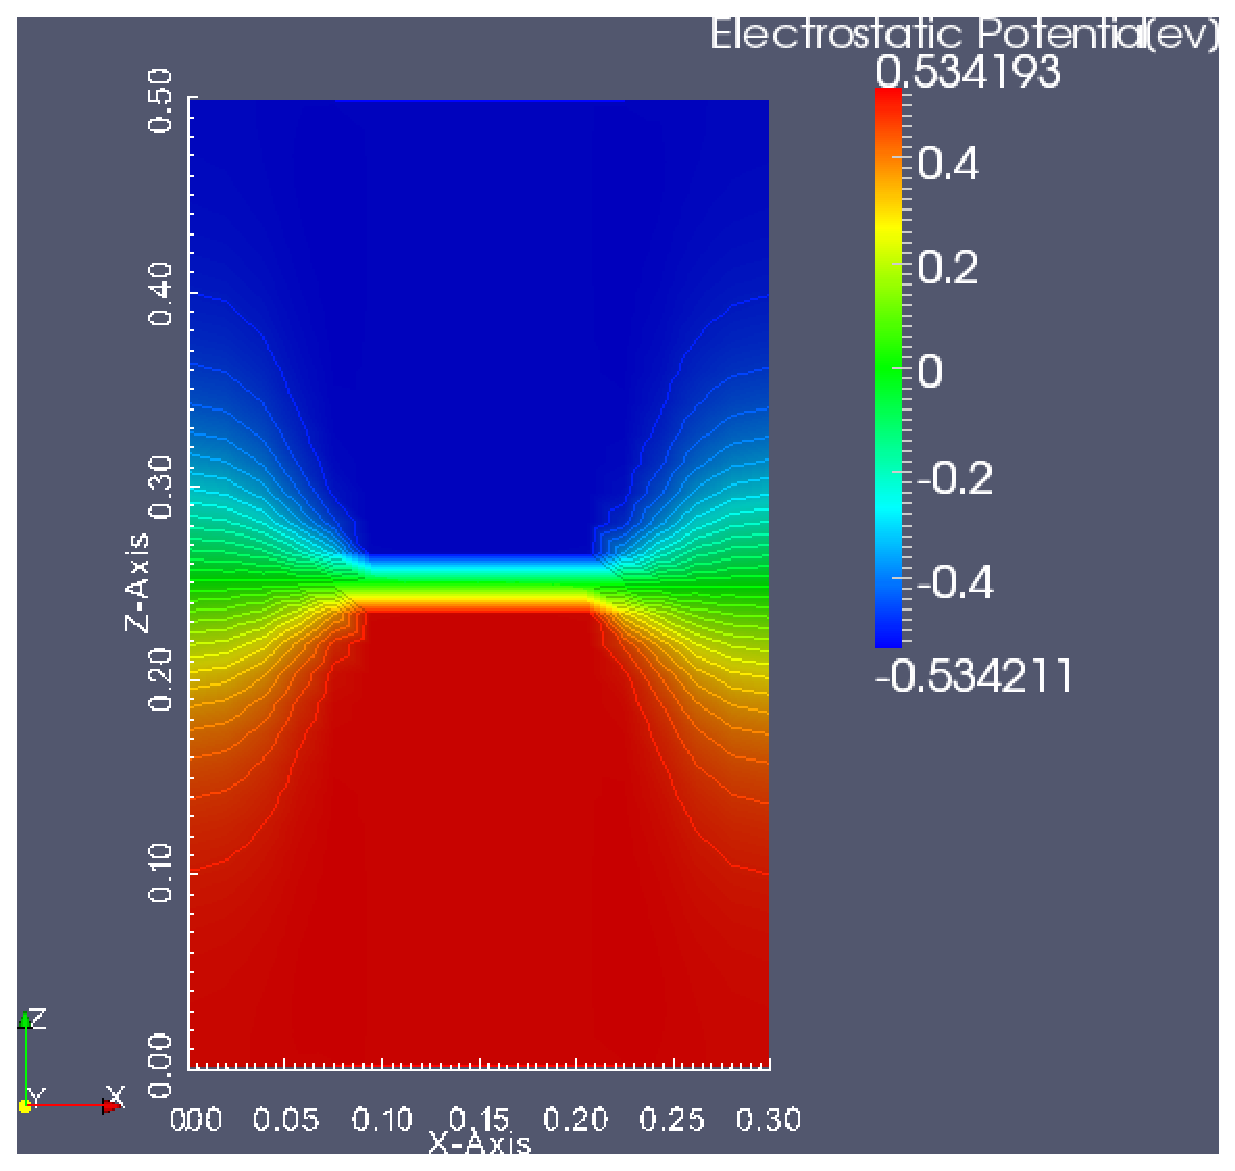
\includegraphics[scale=0.2]{N19P19OX_POT_tool_XZ}}
          \end{figure}
\end{center}
\end{column}

\begin{column}{0.3 \textwidth}
\begin{center}
\begin{figure}[!h]
\subfigure[Sdevice]
          {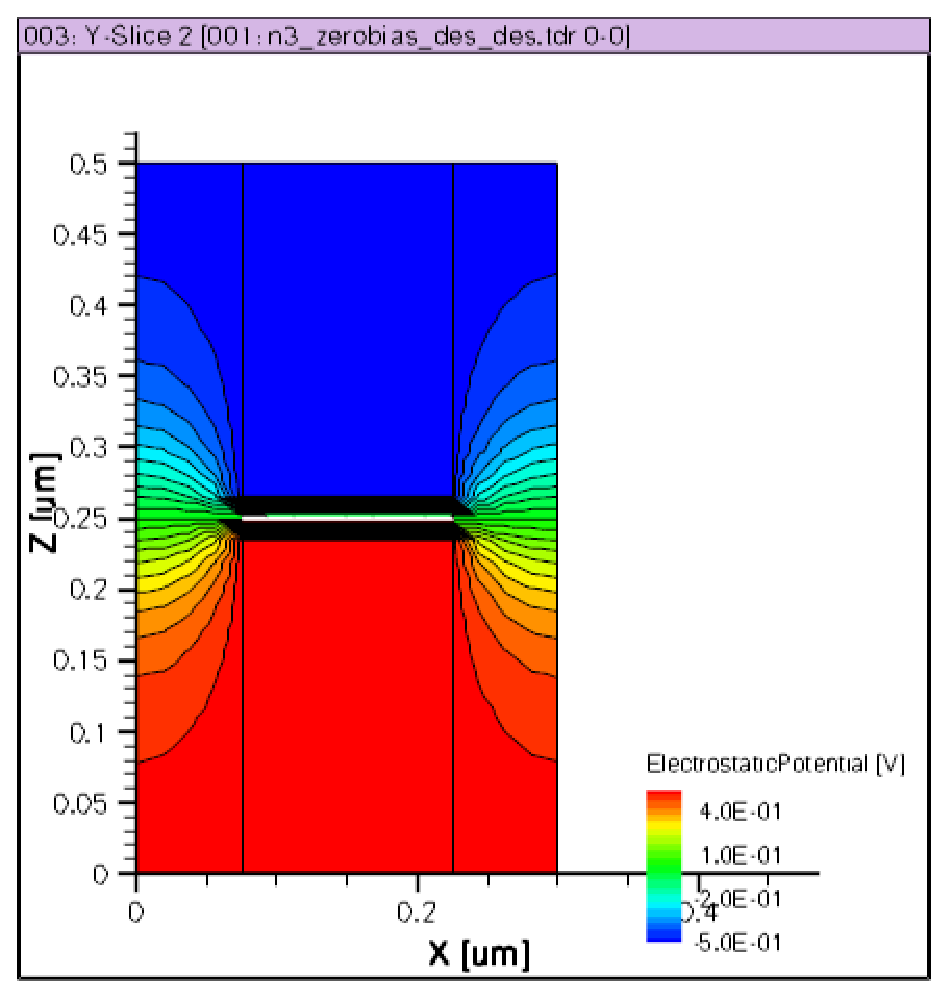
\includegraphics[scale=0.2]{N19P19OX_POT_sdevice_XZ}}
\end{figure}
\end{center}
\end{column}

\end{columns}

\end{frame}

\begin{frame}
\frametitle{Carica interfacciale - Free Charge N19P19}
Problemi evidenti di carica interfacciale nonostante la soluzione del potenziale sembra essere quella che si avvicini di pi\`u alla soluzione sdevice.
\begin{columns}

\begin{column}{0.3 \textwidth}
\begin{center}
\begin{figure}[!h]
\subfigure[Sezione XZ]
          {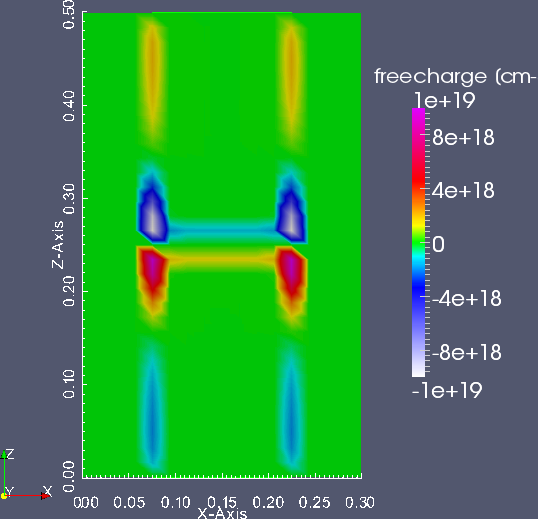
\includegraphics[scale=0.2]{N19P19OX_Q_tool_XZ}}
          \end{figure}
\end{center}
\end{column}

\begin{column}{0.3 \textwidth}
\begin{center}
\begin{figure}[!h]
\subfigure[Sezione YZ]
          {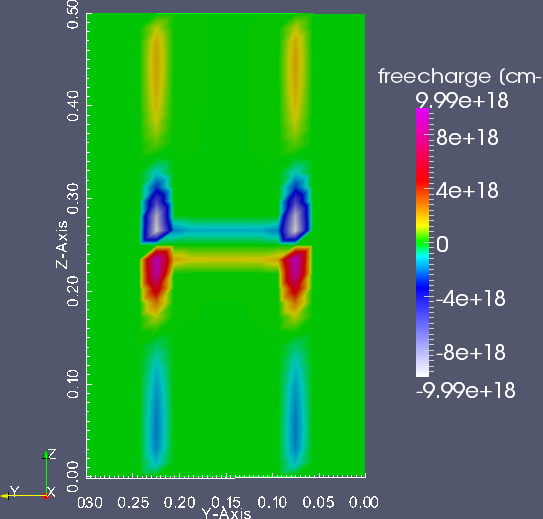
\includegraphics[scale=0.2]{N19P19OX_Q_tool_YZ}}
\end{figure}
\end{center}
\end{column}

\begin{column}{0.3 \textwidth}
\begin{center}
\begin{figure}[!h]
\subfigure[Sdevice]
          {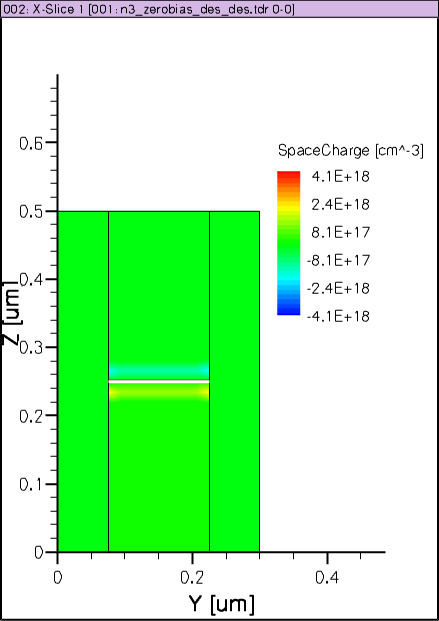
\includegraphics[scale=0.2]{N19P19OX_Q_sdevice_YZ}}
\end{figure}
\end{center}
\end{column}

\end{columns}

\end{frame}


\begin{frame}
\frametitle{Conclusioni}
\begin{itemize}
\item[1.] Il solutore non lineare di Poisson sul silicio \`e allineato con i risultati di sdevice.
\item[2.] Il solutore lineare di Poisson su ossido \`e allineato con i risultati di sdevice
\item[3.] Il solutore non lineare di Poisson applicato alla situazione silicio-ossido non d\`a soluzioni corrette: viste le conclusioni precedenti il problema \`e legato al trattamento dell'interfaccia silicio-ossido. 
\end{itemize}
\end{frame}

\section{New results}
\subsection{N16P16}

\begin{frame}
\tableofcontents[currentsection]
\end{frame}

\begin{frame}
\frametitle{Potenziale N16P16}
\begin{columns}

\begin{column}{0.3 \textwidth}
\begin{center}
\begin{figure}[!h]
         \subfigure[Coeff Si]
          {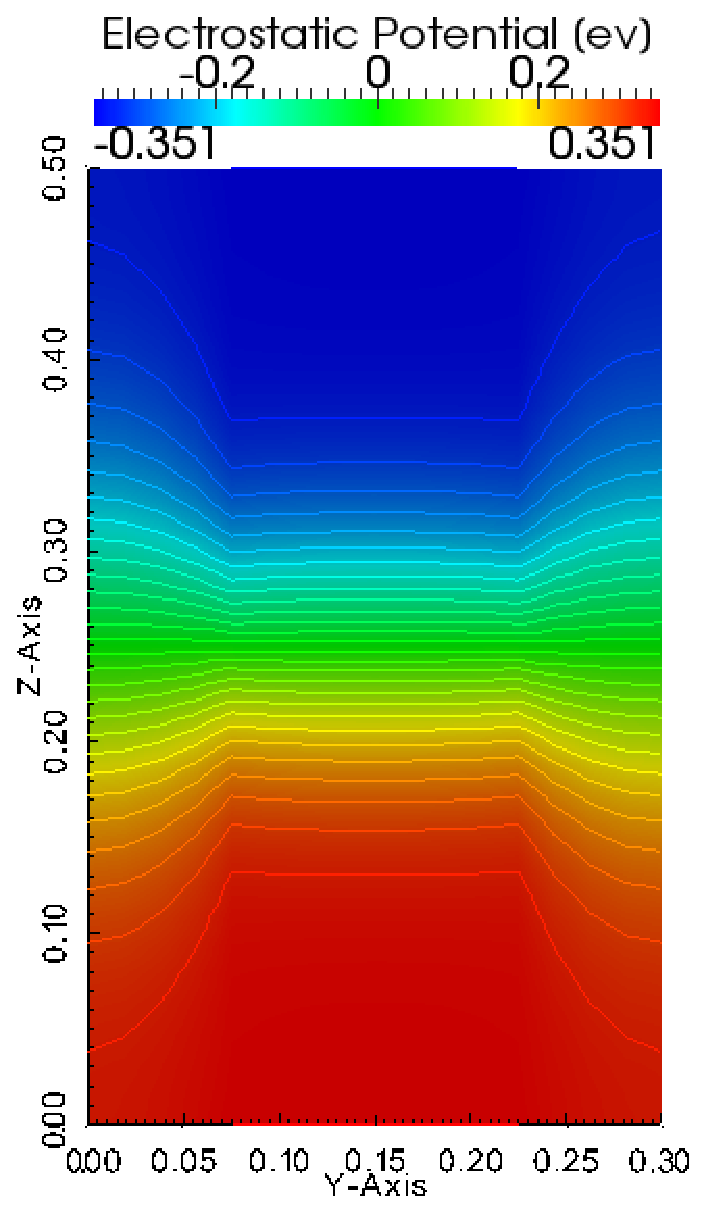
\includegraphics[scale=0.2]{N16P16YZ_coeffSi}}
          \end{figure}
\end{center}
\end{column}

\begin{column}{0.3 \textwidth}
\begin{center}
\begin{figure}[!h]
         \subfigure[Coeff Ox]
          {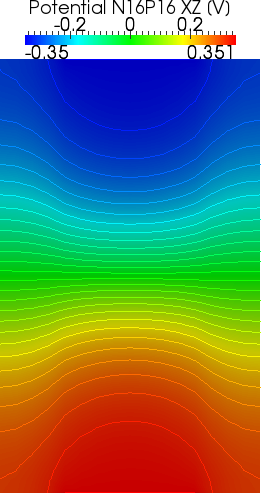
\includegraphics[scale=0.22]{N16P16XZ}}
\end{figure}
\end{center}
\end{column}

\begin{column}{0.3 \textwidth}
\begin{center}
\begin{figure}[!h]
         \subfigure[Sdevice]
          {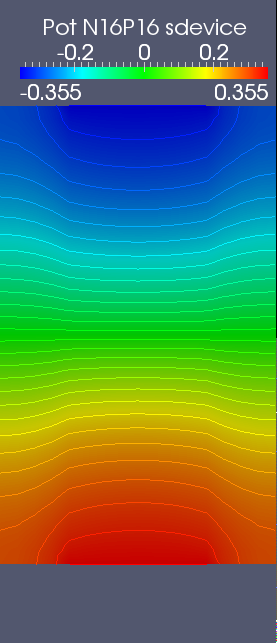
\includegraphics[scale=0.22]{N16P16sdeviceSLICE}}
\end{figure}
\end{center}
\end{column}

\end{columns}

\end{frame}

\begin{frame}
\frametitle{Potenziale tagli N16P16}

\begin{columns}

\begin{column}{0.25 \textwidth}
\begin{center}
\begin{figure}[!h]
         \subfigure[X=Y=0.15]
          {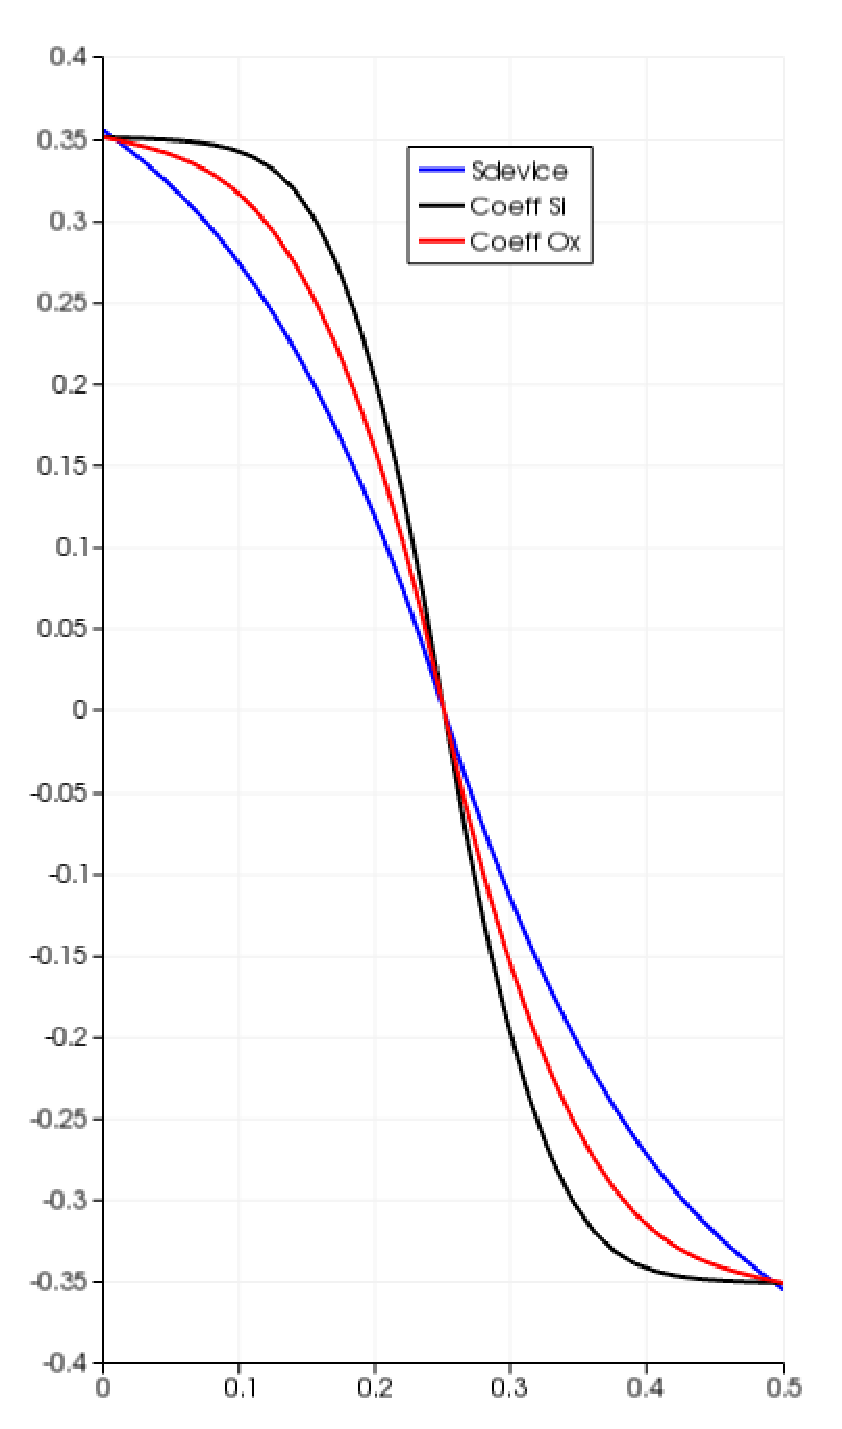
\includegraphics[scale=0.2]{N16P16_POT_Z}}
          \end{figure}
\end{center}
\end{column}

\begin{column}{0.25 \textwidth}
\begin{center}
\begin{figure}[!h]
         \subfigure[X=0.15 Z=0.2]
          {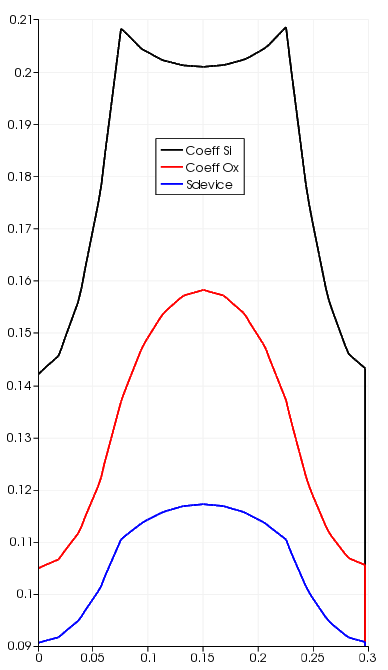
\includegraphics[scale=0.2]{N16P16_POT_Z02}}
\end{figure}
\end{center}
\end{column}

\begin{column}{0.25 \textwidth}
\begin{center}
\begin{figure}[!h]
         \subfigure[X=0.15 Z=0.25]
          {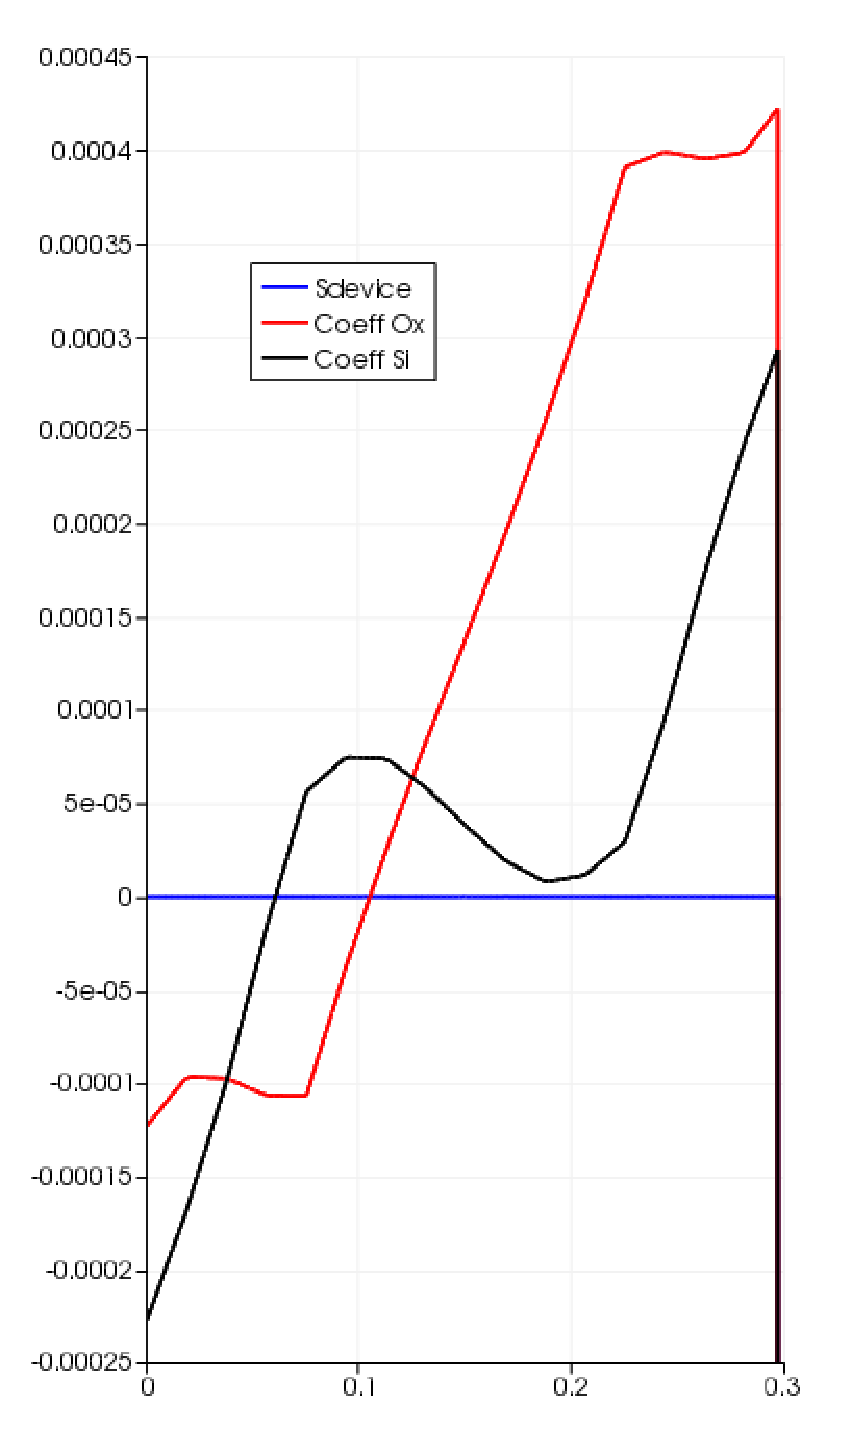
\includegraphics[scale=0.2]{N16P16_POT_Z025}}
\end{figure}
\end{center}
\end{column}

\begin{column}{0.25 \textwidth}
\begin{center}
\begin{figure}[!h]
         \subfigure[X=0.15 Z=0.48]
          {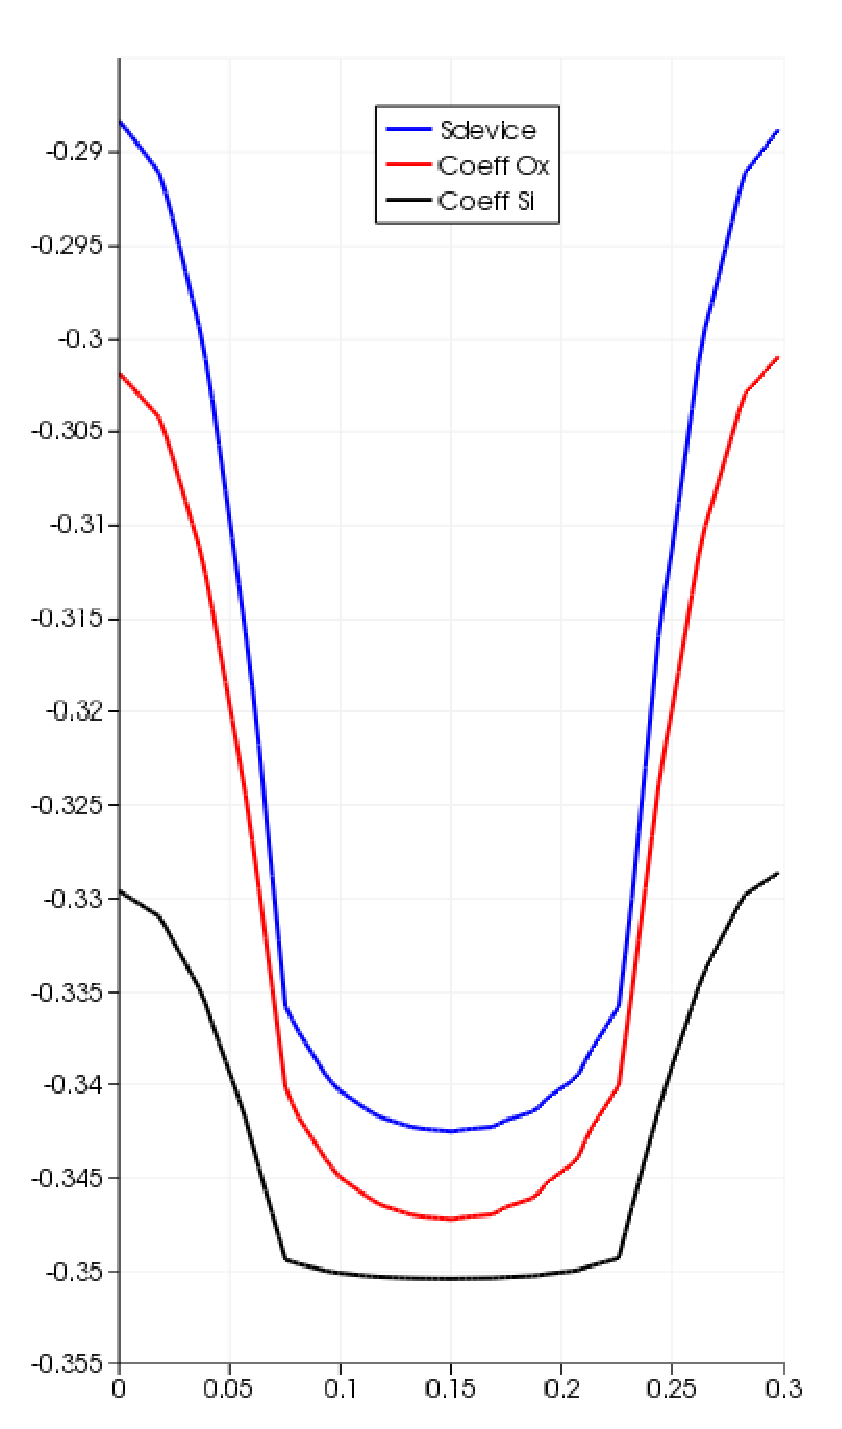
\includegraphics[scale=0.2]{N16P16_POT_Z048}}
\end{figure}
\end{center}
\end{column}

\end{columns}
\end{frame}



%----------------------------------------


\begin{frame}
\frametitle{Potenziale N16P16}
\begin{columns}

\begin{column}{0.3 \textwidth}
\begin{center}
\begin{figure}[!h]
          {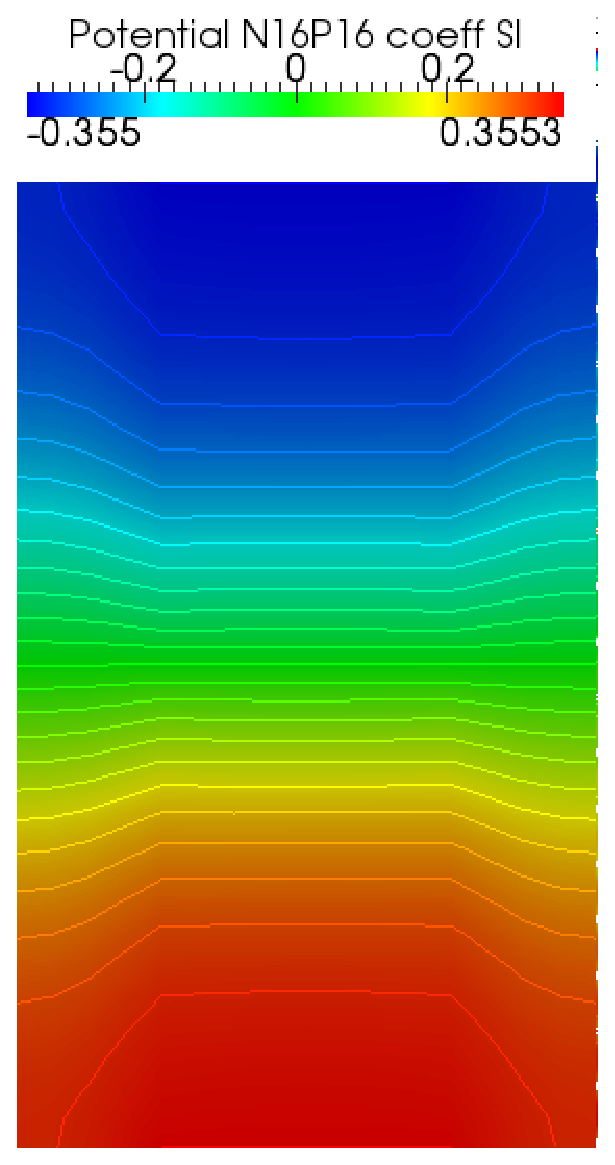
\includegraphics[scale=0.25]{PNOX/N16P16/PotentialCoeffSI}}
          \end{figure}
\end{center}
\end{column}

\begin{column}{0.3 \textwidth}
\begin{center}
\begin{figure}[!h]
          {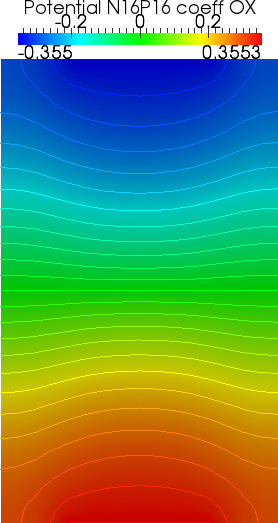
\includegraphics[scale=0.25]{PNOX/N16P16/PotentialCoeffOX}}
\end{figure}
\end{center}
\end{column}

\begin{column}{0.3 \textwidth}
\begin{center}
\begin{figure}[!h]
          {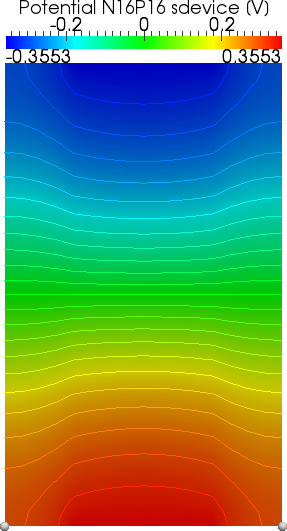
\includegraphics[scale=0.25]{PNOX/N16P16/PotentialSdevice}}
\end{figure}
\end{center}
\end{column}

\end{columns}

\end{frame}

\begin{frame}
\frametitle{Potenziale tagli N16P16}
\begin{columns}

\begin{column}{0.3 \textwidth}
\begin{center}
\begin{figure}[!h]
         \subfigure[X=Y=0.15]
          {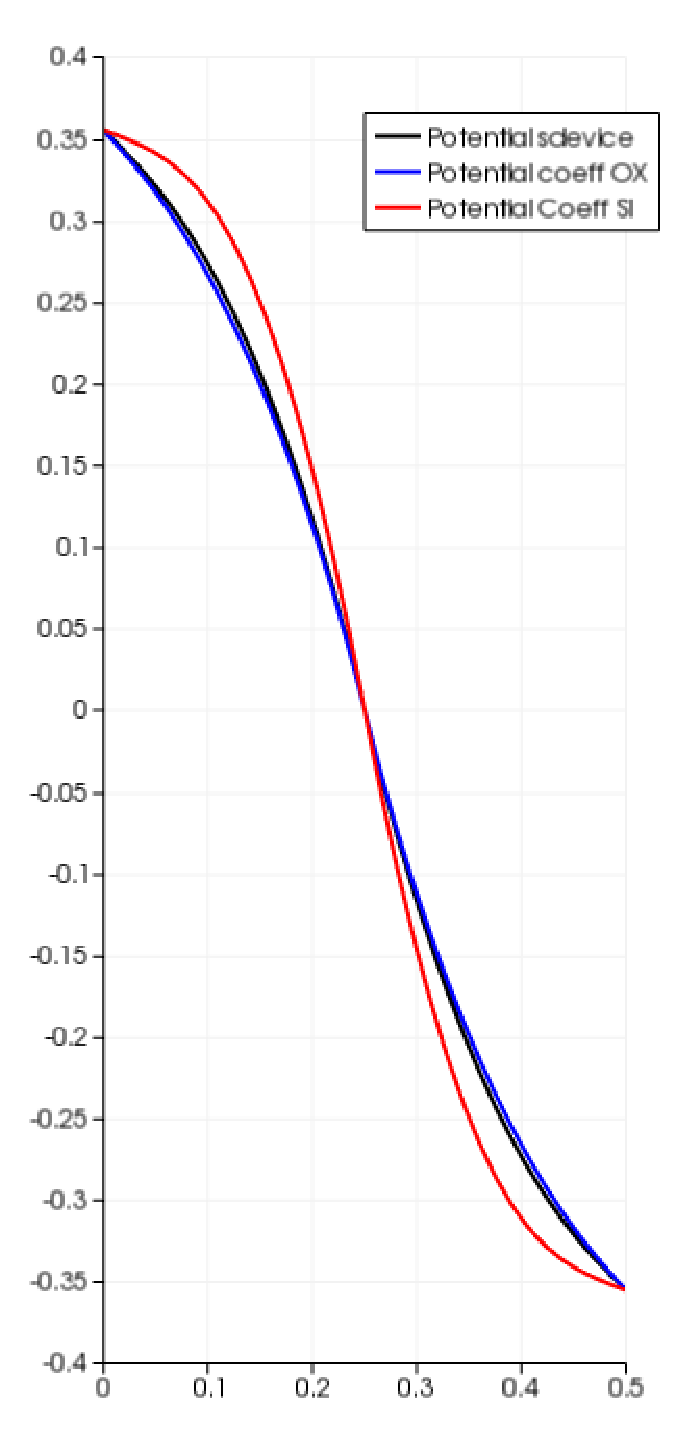
\includegraphics[scale=0.25]{PNOX/N16P16/Pot_Z}}
          \end{figure}
\end{center}
\end{column}

\begin{column}{0.3 \textwidth}
\begin{center}
\begin{figure}[!h]
         \subfigure[X=0.15 Z=0.25]
          {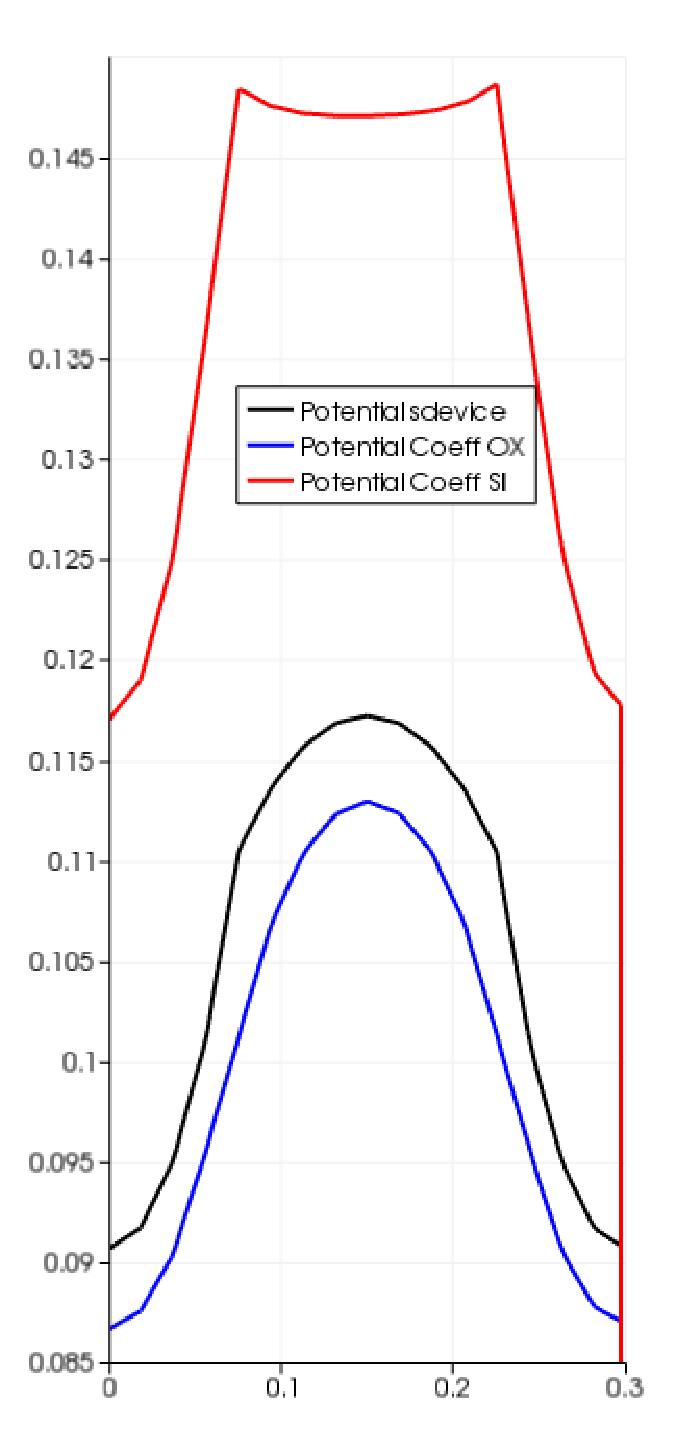
\includegraphics[scale=0.2]{PNOX/N16P16/Pot_Y_Z02}}
\end{figure}
\end{center}
\end{column}

\begin{column}{0.3 \textwidth}
\begin{center}
\begin{figure}[!h]
         \subfigure[X=0.15 Z=0.0]
          {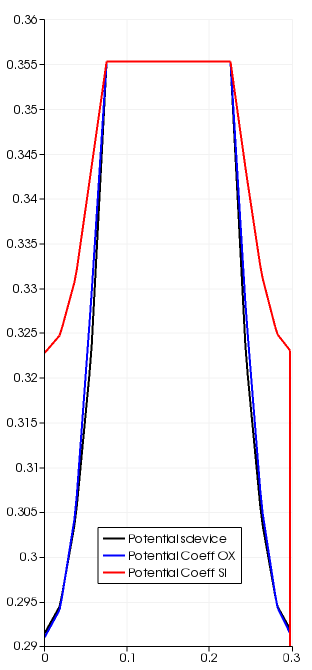
\includegraphics[scale=0.25]{PNOX/N16P16/Pot_Y_Z00}}
\end{figure}
\end{center}
\end{column}

\end{columns}
\end{frame}

\subsection{N19P19}

\begin{frame}
\tableofcontents[currentsection]
\end{frame}

\begin{frame}
\frametitle{Potenziale N19P19}
\begin{columns}

\begin{column}{0.3 \textwidth}
\begin{center}
\begin{figure}[!h]
         \subfigure[Coeff Si]
          {\includegraphics[scale=0.24]{N19P19coeffSiSLICE}}
          \end{figure}
\end{center}
\end{column}

\begin{column}{0.3 \textwidth}
\begin{center}
\begin{figure}[!h]
         \subfigure[Coeff Ox]
          {\includegraphics[scale=0.24]{N19P19coeffOxSLICE}}
\end{figure}
\end{center}
\end{column}

\begin{column}{0.3 \textwidth}
\begin{center}
\begin{figure}[!h]
         \subfigure[Sdevice]
          {\includegraphics[scale=0.24]{N19P19sdeviceSLICE}}
\end{figure}
\end{center}
\end{column}

\end{columns}

\end{frame}


\begin{frame}
\frametitle{Potenziale tagli N19P19}

\begin{columns}

\begin{column}{0.25 \textwidth}
\begin{center}
\begin{figure}[!h]
         \subfigure[Z=0 Y=0.15]
          {\includegraphics[scale=0.2]{N19P19_Z00Y015}}
          \end{figure}
\end{center}
\end{column}

\begin{column}{0.25 \textwidth}
\begin{center}
\begin{figure}[!h]
         \subfigure[Y=0.15 Z=0.2]
          {\includegraphics[scale=0.2]{N19P19_Z02}}
\end{figure}
\end{center}
\end{column}

\begin{column}{0.25 \textwidth}
\begin{center}
\begin{figure}[!h]
         \subfigure[X=0.01 Z=0.2]
          {\includegraphics[scale=0.2]{N19P19_Z02X001}}
\end{figure}
\end{center}
\end{column}

\begin{column}{0.25 \textwidth}
\begin{center}
\begin{figure}[!h]
         \subfigure[X=0.01 Z=0.02]
          {\includegraphics[scale=0.2]{N19P19_Z002Y001}}
\end{figure}
\end{center}
\end{column}

\end{columns}
\end{frame}

%----------------------------------------


\begin{frame}
\frametitle{Potenziale N19P19}
\begin{columns}

\begin{column}{0.3 \textwidth}
\begin{center}
\begin{figure}[!h]
          {\includegraphics[scale=0.25]{PNOX/N19P19/PotentialCoeffSI}}
          \end{figure}
\end{center}
\end{column}

\begin{column}{0.3 \textwidth}
\begin{center}
\begin{figure}[!h]
          {\includegraphics[scale=0.25]{PNOX/N19P19/PotentialCoeffOX}}
\end{figure}
\end{center}
\end{column}

\begin{column}{0.3 \textwidth}
\begin{center}
\begin{figure}[!h]
          {\includegraphics[scale=0.25]{PNOX/N19P19/PotentialSdevice}}
\end{figure}
\end{center}
\end{column}

\end{columns}

\end{frame}

\begin{frame}
\frametitle{Potenziale tagli N19P19}
\begin{columns}

\begin{column}{0.25 \textwidth}
\begin{center}
\begin{figure}[!h]
         \subfigure[X=Y=0.15]
          {\includegraphics[scale=0.2]{PNOX/N19P19/Pot_Y_Z00}}
          \end{figure}
\end{center}
\end{column}

\begin{column}{0.25 \textwidth}
\begin{center}
\begin{figure}[!h]
         \subfigure[X=0.15 Z=0.2]
          {\includegraphics[scale=0.2]{PNOX/N19P19/Pot_Y_Z024}}
\end{figure}
\end{center}
\end{column}

\begin{column}{0.25 \textwidth}
\begin{center}
\begin{figure}[!h]
         \subfigure[X=0.005 Z=0.024]
          {\includegraphics[scale=0.2]{PNOX/N19P19/Pot_Y_Z024X005}}
\end{figure}
\end{center}
\end{column}

\begin{column}{0.25 \textwidth}
\begin{center}
\begin{figure}[!h]
         \subfigure[X=0.0295 Z=0.024]
          {\includegraphics[scale=0.2]{PNOX/N19P19/Pot_Y_Z024X0295}}
\end{figure}
\end{center}
\end{column}

\end{columns}
\end{frame}



\end{document}